% Options for packages loaded elsewhere
\PassOptionsToPackage{unicode}{hyperref}
\PassOptionsToPackage{hyphens}{url}
\documentclass[
  12pt,
]{article}
\usepackage{xcolor}
\usepackage[top=20mm, left=20mm, right=20mm, bottom=20mm]{geometry}
\usepackage{amsmath,amssymb}
\setcounter{secnumdepth}{5}
\usepackage{iftex}
\ifPDFTeX
  \usepackage[T1]{fontenc}
  \usepackage[utf8]{inputenc}
  \usepackage{textcomp} % provide euro and other symbols
\else % if luatex or xetex
  \usepackage{unicode-math} % this also loads fontspec
  \defaultfontfeatures{Scale=MatchLowercase}
  \defaultfontfeatures[\rmfamily]{Ligatures=TeX,Scale=1}
\fi
\usepackage{lmodern}
\ifPDFTeX\else
  % xetex/luatex font selection
\fi
% Use upquote if available, for straight quotes in verbatim environments
\IfFileExists{upquote.sty}{\usepackage{upquote}}{}
\IfFileExists{microtype.sty}{% use microtype if available
  \usepackage[]{microtype}
  \UseMicrotypeSet[protrusion]{basicmath} % disable protrusion for tt fonts
}{}
\makeatletter
\@ifundefined{KOMAClassName}{% if non-KOMA class
  \IfFileExists{parskip.sty}{%
    \usepackage{parskip}
  }{% else
    \setlength{\parindent}{0pt}
    \setlength{\parskip}{6pt plus 2pt minus 1pt}}
}{% if KOMA class
  \KOMAoptions{parskip=half}}
\makeatother
\usepackage{color}
\usepackage{fancyvrb}
\newcommand{\VerbBar}{|}
\newcommand{\VERB}{\Verb[commandchars=\\\{\}]}
\DefineVerbatimEnvironment{Highlighting}{Verbatim}{commandchars=\\\{\}}
% Add ',fontsize=\small' for more characters per line
\usepackage{framed}
\definecolor{shadecolor}{RGB}{248,248,248}
\newenvironment{Shaded}{\begin{snugshade}}{\end{snugshade}}
\newcommand{\AlertTok}[1]{\textcolor[rgb]{0.94,0.16,0.16}{#1}}
\newcommand{\AnnotationTok}[1]{\textcolor[rgb]{0.56,0.35,0.01}{\textbf{\textit{#1}}}}
\newcommand{\AttributeTok}[1]{\textcolor[rgb]{0.13,0.29,0.53}{#1}}
\newcommand{\BaseNTok}[1]{\textcolor[rgb]{0.00,0.00,0.81}{#1}}
\newcommand{\BuiltInTok}[1]{#1}
\newcommand{\CharTok}[1]{\textcolor[rgb]{0.31,0.60,0.02}{#1}}
\newcommand{\CommentTok}[1]{\textcolor[rgb]{0.56,0.35,0.01}{\textit{#1}}}
\newcommand{\CommentVarTok}[1]{\textcolor[rgb]{0.56,0.35,0.01}{\textbf{\textit{#1}}}}
\newcommand{\ConstantTok}[1]{\textcolor[rgb]{0.56,0.35,0.01}{#1}}
\newcommand{\ControlFlowTok}[1]{\textcolor[rgb]{0.13,0.29,0.53}{\textbf{#1}}}
\newcommand{\DataTypeTok}[1]{\textcolor[rgb]{0.13,0.29,0.53}{#1}}
\newcommand{\DecValTok}[1]{\textcolor[rgb]{0.00,0.00,0.81}{#1}}
\newcommand{\DocumentationTok}[1]{\textcolor[rgb]{0.56,0.35,0.01}{\textbf{\textit{#1}}}}
\newcommand{\ErrorTok}[1]{\textcolor[rgb]{0.64,0.00,0.00}{\textbf{#1}}}
\newcommand{\ExtensionTok}[1]{#1}
\newcommand{\FloatTok}[1]{\textcolor[rgb]{0.00,0.00,0.81}{#1}}
\newcommand{\FunctionTok}[1]{\textcolor[rgb]{0.13,0.29,0.53}{\textbf{#1}}}
\newcommand{\ImportTok}[1]{#1}
\newcommand{\InformationTok}[1]{\textcolor[rgb]{0.56,0.35,0.01}{\textbf{\textit{#1}}}}
\newcommand{\KeywordTok}[1]{\textcolor[rgb]{0.13,0.29,0.53}{\textbf{#1}}}
\newcommand{\NormalTok}[1]{#1}
\newcommand{\OperatorTok}[1]{\textcolor[rgb]{0.81,0.36,0.00}{\textbf{#1}}}
\newcommand{\OtherTok}[1]{\textcolor[rgb]{0.56,0.35,0.01}{#1}}
\newcommand{\PreprocessorTok}[1]{\textcolor[rgb]{0.56,0.35,0.01}{\textit{#1}}}
\newcommand{\RegionMarkerTok}[1]{#1}
\newcommand{\SpecialCharTok}[1]{\textcolor[rgb]{0.81,0.36,0.00}{\textbf{#1}}}
\newcommand{\SpecialStringTok}[1]{\textcolor[rgb]{0.31,0.60,0.02}{#1}}
\newcommand{\StringTok}[1]{\textcolor[rgb]{0.31,0.60,0.02}{#1}}
\newcommand{\VariableTok}[1]{\textcolor[rgb]{0.00,0.00,0.00}{#1}}
\newcommand{\VerbatimStringTok}[1]{\textcolor[rgb]{0.31,0.60,0.02}{#1}}
\newcommand{\WarningTok}[1]{\textcolor[rgb]{0.56,0.35,0.01}{\textbf{\textit{#1}}}}
\usepackage{graphicx}
\makeatletter
\newsavebox\pandoc@box
\newcommand*\pandocbounded[1]{% scales image to fit in text height/width
  \sbox\pandoc@box{#1}%
  \Gscale@div\@tempa{\textheight}{\dimexpr\ht\pandoc@box+\dp\pandoc@box\relax}%
  \Gscale@div\@tempb{\linewidth}{\wd\pandoc@box}%
  \ifdim\@tempb\p@<\@tempa\p@\let\@tempa\@tempb\fi% select the smaller of both
  \ifdim\@tempa\p@<\p@\scalebox{\@tempa}{\usebox\pandoc@box}%
  \else\usebox{\pandoc@box}%
  \fi%
}
% Set default figure placement to htbp
\def\fps@figure{htbp}
\makeatother
% definitions for citeproc citations
\NewDocumentCommand\citeproctext{}{}
\NewDocumentCommand\citeproc{mm}{%
  \begingroup\def\citeproctext{#2}\cite{#1}\endgroup}
\makeatletter
 % allow citations to break across lines
 \let\@cite@ofmt\@firstofone
 % avoid brackets around text for \cite:
 \def\@biblabel#1{}
 \def\@cite#1#2{{#1\if@tempswa , #2\fi}}
\makeatother
\newlength{\cslhangindent}
\setlength{\cslhangindent}{1.5em}
\newlength{\csllabelwidth}
\setlength{\csllabelwidth}{3em}
\newenvironment{CSLReferences}[2] % #1 hanging-indent, #2 entry-spacing
 {\begin{list}{}{%
  \setlength{\itemindent}{0pt}
  \setlength{\leftmargin}{0pt}
  \setlength{\parsep}{0pt}
  % turn on hanging indent if param 1 is 1
  \ifodd #1
   \setlength{\leftmargin}{\cslhangindent}
   \setlength{\itemindent}{-1\cslhangindent}
  \fi
  % set entry spacing
  \setlength{\itemsep}{#2\baselineskip}}}
 {\end{list}}
\usepackage{calc}
\newcommand{\CSLBlock}[1]{\hfill\break\parbox[t]{\linewidth}{\strut\ignorespaces#1\strut}}
\newcommand{\CSLLeftMargin}[1]{\parbox[t]{\csllabelwidth}{\strut#1\strut}}
\newcommand{\CSLRightInline}[1]{\parbox[t]{\linewidth - \csllabelwidth}{\strut#1\strut}}
\newcommand{\CSLIndent}[1]{\hspace{\cslhangindent}#1}
\setlength{\emergencystretch}{3em} % prevent overfull lines
\providecommand{\tightlist}{%
  \setlength{\itemsep}{0pt}\setlength{\parskip}{0pt}}
\usepackage{bookmark}
\IfFileExists{xurl.sty}{\usepackage{xurl}}{} % add URL line breaks if available
\urlstyle{same}
\hypersetup{
  pdftitle={The effect of tablet error on the precision of estimating the absolute abundance of microfossils in the FOVS method},
  pdfauthor={Menghan Fu},
  hidelinks,
  pdfcreator={LaTeX via pandoc}}

\title{\textbf{The effect of tablet error on the precision of estimating
the absolute abundance of microfossils in the FOVS method}}
\author{Menghan Fu}
\date{2026-06-24}

\begin{document}
\maketitle

\newtheorem{theorem}{Theorem}

Project supervisor: Anthony Mays

\section{Declaration}\label{declaration}

In submitting this work I am indicating that I have read the
University's Academic Integrity Policy. I declare that all material in
this assessment is my own work except where there is clear
acknowledgement and reference to the work of others. I give permission
for this work to be reproduced and submitted to other academic staff for
educational purposes.

\section{Abstract}\label{abstract}

The FOVS method estimates the absolute abundance of microfossils by
using exotic marker tablets. However, the number of markers contained in
each tablet varies, which may reduce the precision of the concentration
estimates. This study employs repeated simulations to investigate the
impact of tablet dose variation on FOVS precision, whether the influence
could be mitigated through experimental design, and how the relative
importance of tablet errors changes under different conditions. Three
scenarios are respectively set up: tablet coefficient of variation (CV),
number of tablets, and target-to-marker ratio. Each group of parameters
is simulated 5,000 times. The results show that as tablet CV increases,
the total theoretical error and the importance of tablet error also
increase. Increasing the tablet number can reduce tablet errors and
improve estimation precision. The relative importance of tablet errors
is also influenced by the target-to-marker ratio: when there are more
markers, tablet errors may become the main source of error; when there
are fewer markers, the error in marker counting will mask its influence.

\section{Introduction}\label{introduction}

Microfossils can record changes in past biological communities and
environments, and thus are often used in the study of ancient
environments and ecosystems (Mays, Amores, and Mays (2025), p.~2). Many
studies use relative abundance to describe the proportions of different
microfossil types in a sample, but changes in the proportion do not
necessarily indicate a change in the actual quantity, because a change
in the quantity of one type will also affect the proportion of other
types (Jackson (1997), p.~929--932). Absolute abundance can provide the
actual number of microfossils in a single sample, thereby enabling a
more direct comparison between different samples (Mays, Amores, and Mays
(2025), p.~2). However, ordinary quadrat sampling can only observe a
small portion of the area on the prepared slides, making it difficult to
directly convert the counts in the field of view into the absolute
abundance in the original sample (Mays, Amores, and Mays (2025), p.~7).
This can be achieved by adding a known number of exotic markers before
sample processing, and then determining the conversion by the ratio of
the target microfossils to the markers (J. Stockmarr (1971), p.~619).
The FOVS method, based on this approach, divides the counting of targets
and markers into two stages to enhance the efficiency of data collection
(Mays, Amores, and Mays (2025), p.~6--8).

In practical applications, markers are usually introduced by tablets,
but the number of markers in each tablet is not exactly the same and
there are variations (J. Stockmarr (1973), p.~89; Maher (1981),
p.~158--159). This tablet dose variation causes the actual marker dose
to deviate from the nominal dose used in the calculation, which may
affect the precision of the absolute abundance estimation. Therefore,
this study focuses on tablet dose variation, and mainly examines the
following three questions: How does tablet dose variation affect the
precision of absolute abundance estimation in FOVS method? If the effect
is substantial, can it be reduced through changes in experimental
design? How does this impact of tablet dose variation vary under
different experimental conditions? To address these questions, this
study uses simulated data to establish three scenarios that change the
marker dose variation in the tablets, the number of tablets added, and
the target-to-marker ratio in the sample. For each scenario, we compare
the final concentration estimate and its theoretical error. The total
error is further separated into its different components for analysis,
and the effort required to complete the counts is also recorded.

\section{Background}\label{background}

\subsection{Exotic marker method}\label{exotic-marker-method}

The concentration of microfossils is usually expressed as the number of
target particles per unit mass, area or volume of the sediment (Mays,
Amores, and Mays (2025), p.~3, Eqn. 1). Since the sediment needs to
undergo experimental treatment, and a portion of the treated material is
then used to make microscope slides, the particle distribution and
concentration on the slides are no longer the same as those in the
original sediment. Therefore, ordinary quadrat sampling can only
estimate the particle density on the slide, but it cannot separately
convert this density into the concentration in the original sample
(Mays, Amores, and Mays (2025), p.~7).

However, using exotic markers can solve this problem. The method of
calculating pollen and spore density by adding a known amount of
exogenous pollen or spores to the sample can be traced back to
Benninghoff (1962). First, measure the mass, area or volume of the
original sample, and then add a known number of exotic markers. The
processed samples are made into slides, and then the target particles
and markers are counted simultaneously under the microscope. Since the
number of markers added to the sample is known, and this method assumes
that the targets and markers are fully mixed in the treated sample and
are similarly affected during the treatment process, the
target-to-marker ratio observed on the slide can approximately represent
the proportion in the entire sample (Mays, Amores, and Mays (2025),
p.~2--3). This is thereby used to estimate the concentration of the
target particles in the original sample.

Following Mays, Amores, and Mays (2025) (p.~3, Eqn. 1), the
concentration of target microfossils is calculated as:

\begin{align}
\label{eqn:c} c = \frac{xN_1\bar{Y}_1}{nV},
\end{align}

where, \(c\) represents the concentration of the target in the original
sample; \(x\) is the number of targets counted; \(n\) is the number of
markers counted; \(N_1\) is the number of doses (e.g., tablets) of
markers added to the sample; \(\bar{Y}_1\) is the average number of
markers per dose; \(V\) is the total size (mass, area or volume) of
sample. Therefore, \(\frac{x}{n}\) represents the target-to-marker ratio
within the counting area, while \(N_1\bar{Y}_1\) is the nominal total
number of markers added to the sample. When these two values are
combined, the relative counts on the slide can be converted into the
concentration of the original sample.

\subsection{Tablet and tablet error}\label{tablet-and-tablet-error}

J. Stockmarr (1971) introduced tablets containing a known quantity of
spores from the genus Lycopodium into absolute pollen analysis, enabling
exotic marker particles to be added to the samples at a standardized
dose. Each tablet is composed of a certain number of Lycopodium spores
and a soluble carrier; after the addition of the sample, the carrier
dissolves, while the spores, as identifiable exotic markers, participate
in the subsequent experimental processing and microscopic counting.
Since the spores of Lycopodium are usually easily distinguishable from
the target microfossils in the sample, and can undergo the same chemical
treatment and preparation process as the target particles, the tablets
not only provide an internal standard for concentration calculation, but
also can to some extent reflect the loss of particles during the
experimental treatment process (J. Stockmarr (1971), p.~615--619; Mays,
Amores, and Mays (2025), p.~2--3).

However, the actual number of spores in each tablet is not exactly the
same. A tablet batch can therefore be described using its mean marker
dose and standard deviation. Therefore, in the concentration formula,
\(N_1\bar{Y}_1\) represents the nominal value, and the actual total
number of markers added may be higher or lower than this value (J.
Stockmarr (1973), p.~89, Fig. 2; Maher (1981), pp.~158--159).

The random variation between this actual marker dose and its nominal
value is referred to as tablet error in this study. Tablet error is
measured as the coefficient of variation of marker dose per tablet:

\begin{align}
\label{eqn:CVT} CV_T = \frac{\sigma_T}{\bar{Y}_1},
\end{align}

where, \(\sigma_T\) represents the standard deviation of the number of
markers per tablet, and \(\bar{Y}_1\) is as in Eqn \eqref{eqn:c} .

\subsection{FOVS method}\label{fovs-method}

In the normal exotic marker method, the slide is typically scanned
continuously while both targets and markers are counted until a
predetermined number of particles of one type is reached. When the
number of targets and markers is relatively close, this method is more
effective; however, when the number of targets is much greater than that
of markers, it is necessary to count a large number of targets in order
to observe a sufficient number of rare markers (Price et al. (2016),
p.~78--79, 86 and 89, Fig. 3). At this point, further increasing the
target count offers limited assistance in improving precision, but it
will increase the workload required for microscope counting.

Mays, Amores, and Mays (2025) proposed the field-of-view subsampling
(FOVS) method, which divides the counting of targets and markers into
two stages. First, perform the calibration count (Mays, Amores, and Mays
(2025), p.~7): Count all the targets in selected microscope fields of
view and estimate the average number of targets for each field of view.
For example, if there are 20 calibration fields and 100 targets are
counted within them, the average number of targets per field is 5. Then,
perform the extrapolation count (Mays, Amores, and Mays (2025),
p.~7--8): Observe a large number of new fields, and mainly count the
markers. In this way, targets do not need to be counted individually in
each extrapolation field. Instead, the average value obtained from the
calibration count can be used for estimation.

The total number of targets in the extrapolation fields is estimated by
(Mays, Amores, and Mays (2025), p.~7, Eqn. 3)

\begin{align}
\label{eqn:hatx} \hat{x}=\bar{Y}_xN_E,
\end{align}

where, \(\hat{x}\) is the estimated total number of targets in the
extrapolation fields; \(\bar{Y}_x\) is the average number of targets per
calibration field; \(N_E\) is the number of extrapolation fields.
Replacing the direct target count \(x\) in the Equation \eqref{eqn:c}
with \(\hat{x}\), we can obtain the FOVS concentration estimate (Mays,
Amores, and Mays (2025), p.~8, Eqn. 4):

\begin{align}
\label{eqn:cFx} c_{F_x}=\frac{\hat{x}N_1\bar{Y}_1}{nV},
\end{align}

where, \(c_{F_x}\) represents the concentration of target microfossils
obtained by the FOVS method; \(\hat{x}\) is as in Eqn \eqref{eqn:hatx};
\(n\) is the number of markers counted in the extrapolation count;
\(N_1\), \(\bar{Y}_1\), \(V\) are as in Eqn \eqref{eqn:c}.

\subsection{Error structure in FOVS
method}\label{error-structure-in-fovs-method}

The precision of FOVS concentration estimates is expressed by the total
standard error, and a smaller value indicates a higher precision in
concentration estimates. The total error of FOVS is composed of three
sources: the variation of marker dose in the tablets, the sampling
variation of target density in the calibration fields, and the counting
variation of marker quantity in the extrapolation count. Assuming that
these three sources of error are independent of each other, the total
error can be expressed as (Mays, Amores, and Mays (2025), p.~8, Eqn. 5):

\begin{align}
\label{eqn:sigmaFx} \sigma_{Fx} = 100 \sqrt{\left(\frac{s_{1P}}{\sqrt{N_1}}\right)^2 + \left(\frac{s_{3P}}{\sqrt{N_{C}}}\right)^2 + \left(\frac{\sqrt{n}}{n}\right)^2},
\end{align}

where, \(\sigma_{F_x}\) is the total standard error of the mean
concentration for the FOVS method (in \%); \(s_{1P}\) represents the
proportional standard deviation of the marker quantity per tablet,
corresponding to \(CV_T\) in this study; \(N_1\) is as in Eqn
\eqref{eqn:c}; \(s_{3P}\) is the proportional standard deviation of the
target count per calibration field of view; \(N_C\) is the number of
calibration fields; \(n\) is as in Eqn \eqref{eqn:cFx}.

For clarity of interpretation, the three error components can be
expressed separately as:

\begin{align}
\label{eqn:error_term} E_T=100\frac{s_{1P}}{\sqrt{N_1}}, \qquad E_C=100\frac{s_{3P}}{\sqrt{N_C}}, \qquad E_M=100\frac{1}{\sqrt{n}}, 
\end{align}

where, \(E_T\), \(E_C\) and \(E_M\) respectively represent the tablet
error term, calibration error term and marker counting error term.

\subsection{Data-collection effort in FOVS
method}\label{data-collection-effort-in-fovs-method}

However, the improvement in precision should also be balanced against
the associated effort. Increasing the number of particles or the number
of fields of view usually improves the estimation precision, but it may
also increase the time required for microscope observation. Mays,
Amores, and Mays (2025) (p.~10--11, Eqn. 7) expressed the FOVS method
effort as the sum of the particle-counting effort and the microscope
field-of-view moving effort. The formula is

\begin{align}
\label{eqn:eF} e_F=(\omega N_C)+x+(\omega N_E)+n, 
\end{align}

where, \(e_F\) is the FOVS data collection effort; \(N_C\) is as in Eqn
\eqref{eqn:sigmaFx}; \(N_E\) is as in Eqn \eqref{eqn:hatx}; \(x\) is the
total number of targets counted in the calibration count; \(n\) is as in
Eqn \eqref{eqn:cFx}; \(\omega\) is the field-of-view transition effort
factor. Following Mays, Amores, and Mays (2025) (p.~11), moving to a new
field of view is treated as requiring the same effort as counting two
individual particles, so the fov transition effort factor is fixed at
\(\omega=2\) in all simulations. Therefore, \((\omega N_C) + x\)
represents the effort of the calibration count, and \((\omega N_E) + n\)
represents the effort of the extrapolation count.

\section{Methods}\label{methods}

The current studies have separately examined the marker dose variations
of tablet and their statistical properties, and have also established a
theoretical framework for FOVS concentration, error and effort. However,
the studies reviewed here have not explicitly quantified how tablet dose
variation affects precision within the FOVS framework, and it is also
unclear at present under what conditions the tablet error will become a
significant source of error. Therefore, this study examines tablet CV,
tablet number, and target-to-marker ratio in three simulated scenarios
to quantify the impact of tablet errors on the total error, and to
compare the relative influence of tablet errors with other error sources
on the total error.

\subsection{Overall simulation
framework}\label{overall-simulation-framework}

This study uses repeated random simulation to investigate the impact of
tablet errors on the precision of FOVS concentration estimates.

Each simulation is carried out following the steps below:

\begin{quote}
\begin{itemize}
\tightlist
\item
  Step 1: The simulation area is a square with a side length of 1. Each
  simulation generates 10,000 targets. The x-coordinate and y-coordinate
  of each target are independently randomly generated between 0 and 1.
  Therefore, each position within the area has an equal chance of being
  selected.
\end{itemize}
\end{quote}

\begin{quote}
\begin{itemize}
\tightlist
\item
  Step 2: For each tablet, the actual marker dose is independently
  generated from a normal distribution with a mean of \(\bar{Y}_1\) and
  a standard deviation of \(\bar{Y}_1CV_T\), based on the relationship
  defined in Equation \eqref{eqn:CVT}. The generated dose is rounded to
  the nearest integer and is limited to at least 1 marker. Then, the
  actual doses of all the tablets are added together to obtain the total
  number of markers actually added in this simulation.
\end{itemize}
\end{quote}

\begin{quote}
\begin{itemize}
\tightlist
\item
  Step 3: Based on the actual total number of markers obtained from this
  simulation, randomly generate the positions of the markers within the
  same square area. The marker and the target are independent of each
  other, and each position within the area has an equal chance of being
  selected.
\end{itemize}
\end{quote}

(See ``Simulation settings and target generation'' and ``Tablet dose
variation and marker generation'' in Appendix A.1 and A.2. These steps
were implemented in the function \texttt{simulate\_fovs\_once()} on
lines 6--44 of \texttt{sims\_Fossil.R}. The simulation parameters and
target locations are defined on lines 6--28, while the nominal marker
dose, random tablet doses, actual marker total, and marker locations are
generated on lines 30--44.)

\begin{quote}
\begin{itemize}
\tightlist
\item
  Step 4: Each field of view (FOV) is a square with a side length of
  0.1. Therefore, the simulation area is divided into \(10 \times 10\)
  FOVs, excluding the outermost ring. Subsequently, a random
  \(7 \times 6\) block containing 42 candidate FOVs is then randomly
  selected from this internal grid. From these candidates, 20 FOVs are
  randomly selected without replacement for the calibration count and
  another 20 non-overlapping FOVs for extrapolation counts.
\end{itemize}
\end{quote}

\begin{quote}
\begin{itemize}
\tightlist
\item
  Step 5: Count the targets in each of the 20 calibration FOVs.
  Particles that fall on the left or bottom boundary of the FOV are
  counted, while those that fall on the right or top boundary are not
  counted to avoid double-counting of particles located on adjacent
  boundaries. Then estimate the average value of the targets in each
  FOV.
\end{itemize}
\end{quote}

\begin{quote}
\begin{itemize}
\tightlist
\item
  Step 6: Count the markers in 20 extrapolation FOVs. As with the
  calibration count method, the left and lower boundaries are included,
  while the right and upper boundaries are excluded.
\end{itemize}
\end{quote}

(See ``FOV grid construction and sampling design'' and ``Target and
marker counting'' in Appendix A.3 and A.4. The FOV grid and the
non-overlapping calibration and extrapolation fields were generated on
lines 46--104 of \texttt{sims\_Fossil.R}. Target and marker particles
within the selected FOVs were counted on lines 106--128 of the same
file.)

\begin{quote}
\begin{itemize}
\tightlist
\item
  Step 7: Using the Equation \eqref{eqn:hatx}, the total number of
  targets within 20 extrapolation FOVs is estimated. Calculate the FOVS
  concentration using the Equation \eqref{eqn:cFx}, and the nominal
  marker dose, \(N_1\bar{Y}_1\), is used rather than the simulated
  actual marker total.
\end{itemize}
\end{quote}

\begin{quote}
\begin{itemize}
\tightlist
\item
  Step 8: Each set of parameters is simulated 5,000 times, and then the
  average values of each output are calculated.
\end{itemize}
\end{quote}

(See ``Concentration, effort and error calculation'' in Appendix A.5 and
``Repeated simulations'' in Appendix B.1. The concentration estimate,
data-collection effort, and theoretical error were calculated in
\texttt{simulate\_fovs\_once()} on lines 130--188 of
\texttt{sims\_Fossil.R}. Each parameter setting was repeated 5,000 times
using \texttt{simulate\_fovs\_repeated()} on lines 193--220.)

\begin{table}[ht!]
\centering
\small
\renewcommand{\arraystretch}{1.5}
\begin{tabular}{
p{0.18\textwidth}
p{0.72\textwidth}
}
\hline
\textbf{Scenario} & \textbf{Parameter settings} \\
\hline

Scenario 1: Tablet CV &
\textit{Varied:} $CV_T=0,\ 0.01,\ 0.03,\ 0.05,\ 0.07,\ 0.09,\ 0.11$.
\newline
\textit{Fixed:} $N_1=1$, $\bar{Y}_1=5{,}000$, and $u=2$. \\

\hline

Scenario 2: Tablet number &
\textit{Varied pairs $(N_1,\bar{Y}_1)$:}
$(1,5{,}000)$,
$(2,2{,}500)$,
$(4,1{,}250)$, and
$(6,833.33)$.
\newline
\textit{Fixed:} $CV_T=0.04$, $N_1\bar{Y}_1=5{,}000$, and $u=2$. \\

\hline

Scenario 3: Target-to-marker ratio &
\textit{Varied pairs $(u,\bar{Y}_1)$:}
$(1,10{,}000)$,
$(2,5{,}000)$,
$(4,2{,}500)$,
$(6,1{,}666.67)$,
$(8,1{,}250)$,
$(10,1{,}000)$, and
$(15,666.67)$.
\newline
\textit{Fixed:} $N_1=1$ and $CV_T=0.04$. \\

\hline

Common settings &
$n_{\mathrm{target}}=10{,}000$, $V=1$, $N_C=N_E=20$ and $R=5{,}000$. \\

\hline
\end{tabular}
\caption{\footnotesize Summary of parameter settings for the three simulation scenarios. The varied and fixed parameters for each scenario are shown.}
\label{tab:scenario-settings}
\end{table}

\subsection{Scenario 1: Varying tablet
CV}\label{scenario-1-varying-tablet-cv}

This scenario regards tablet error as an experimental factor, and by
altering the tablet CV, we observe its effect on the FOVS precision. In
order to systematically compare this effect, seven tablet CV levels are
examined, while other parameters remain unchanged. The specific
parameter settings are summarized in Table \ref{tab:scenario-settings}.
Among them, when tablet CV is 0, it indicates that the marker dose of
each tablet is fixed at the average value, without introducing single
tablet dose variation. At other levels, the actual marker dose per
tablet is randomly generated around the mean value of 5,000 based on the
corresponding CV. Each CV level is simulated 5,000 times, while all
other parameter settings remain unchanged. Therefore, the differences
between the results of each group can be more clearly attributed to the
changes in the tablet CV itself.

(See ``Tablet CV scenario code and output'' in Appendix C.1. The seven
tablet CV levels were defined and simulated on lines 278--300 of
\texttt{sims\_Fossil.R}.)

This section is mainly used to answer how the precision of the FOVS
concentration estimate will change as the tablet dose variation
increases, and whether the influence of the tablet error on the overall
error will gradually increase.

\subsection{Scenario 2: Varying tablet
number}\label{scenario-2-varying-tablet-number}

Apart from tablet CV, the second core variable examined in this study is
\(N_1\), which refers to the number of tablets added to the sample.
Intuitively, if the dose variations per tablet are independent of each
other, then when more tablets are added, the random differences between
individual tablets will be partially averaged out at the overall dose
level. Therefore, the impact of tablet error on the final concentration
estimate should decrease. To verify this, a separate analysis of \(N_1\)
is conducted.

In this scenario, tablet CV is fixed at 0.04, which is based on the
tablet data reported by J. Stockmarr (1973) (p.~89, Fig. 2). Stockmarr
measured 71 tablets from a single production batch and reported the
average marker count is 12,488, with a standard deviation of 499 and a
corresponding CV of 4.0\%. Therefore, in this study it is approximated
as 0.04. To isolate the effect of tablet number from the effect of
marker abundance, the nominal total marker dose is fixed at 5,000.
Therefore, as \(N_1\) increases, the nominal mean marker dose per tablet
unit is calculated as:

\begin{align}
\label{eqn:Ybar1N1} \bar{Y}_1 = \frac{5000}{N_1}.
\end{align}

The paired values of \(N_1\) and \(\bar{Y}_1\) are summarized in Table
\ref{tab:scenario-settings}. This fixed-dose design enables the
variation in theoretical error to be attributed to the number of
independent tablets, rather than changes in the overall marker
abundance.

(See ``N1 scenario code and output'' in Appendix D.1. The four values of
\(N_1\) and their corresponding mean marker doses per tablet were
defined and simulated on lines 303--328 of \texttt{sims\_Fossil.R}.)

This section's analysis addresses another more practical issue: If
tablet errors do indeed affect the FOVS precision, then in the
experimental design, could increasing the number of tablets serve as a
mitigation method?

\subsection{Scenario 3: Varying the target-to-marker
ratio}\label{scenario-3-varying-the-target-to-marker-ratio}

The first two scenarios respectively examine tablet dose variation and
tablet number, but the impact of tablet error on the total error might
also be influenced by the ratio of targets and markers in the sample. In
the FOVS method, estimation precision depends not only on tablet error
but also on the number of markers actually counted in the extrapolation
counts. If there are fewer markers in the sample, a smaller number of
markers will usually be counted during extrapolation counts. A smaller
marker count is more susceptible to random fluctuations, thus increasing
the marker counting error, and the relative contribution of tablet error
in the total error may also change accordingly. Therefore, this study
further establishes a target-to-marker ratio scenario to examine the
overall error structure under different ratios of targets and markers.

The nominal target-to-marker ratio, \(u\), is defined as:

\begin{align}
\label{eqn:u} u = \frac{n_{\mathrm{target}}}{N_1 \bar{Y}_1},
\end{align}

where, \(n_{\mathrm{target}}\) represents the total number of targets,
and \(N_1\bar{Y}_1\) represents the nominal total number of markers.
Since the actual tablet dose in each simulation can vary randomly, the
\(u\) here represents the nominal ratio set based on the average marker
dose. To obtain these ratios, the mean marker dose per tablet is set as:

\begin{align}
\label{eqn:Ybar1u} \bar{Y}_1 = \frac{10000}{u}.
\end{align}

Therefore, as shown in Table \ref{tab:scenario-settings}, the paired
values of \(u\) and \(\bar{Y}_1\) are summarized, and the number of
targets, tablet number, and tablet CV are held constant, while the
nominal marker dose is changed to produce different ratios.

(See ``Target-to-marker ratio scenario code and output'' in Appendix
E.1. The seven ratio levels were defined on lines 331--334 of
\texttt{sims\_Fossil.R}. The corresponding mean marker dose was
calculated for each ratio and the repeated simulations were conducted on
lines 335--358 of the same file.)

This section mainly examines whether the relative importance of tablet
error in total error is constant or whether it changes along with other
error terms.

\subsection{Error decomposition and output
metrics}\label{error-decomposition-and-output-metrics}

\subsubsection{Error decomposition}\label{error-decomposition}

This study also conducts an error decomposition analysis for three
simulation scenarios. Specifically, for each simulation, the tablet
error term, calibration error term and marker counting error term are
calculated separately. Then, the average values of each error term from
the 5,000 simulations are used for comparison. This approach can further
determine which specific source of error is primarily responsible for
the change in the total theoretical error, rather than merely assessing
whether the overall error has changed.

In order to compare the relative importance of the three error
components, their approximate relative contributions to the total
theoretical error are also calculated. For example, the approximate
relative contribution of the tablet error term is calculated as:

\begin{align}
\label{eqn:ST} S_T = \frac{\bar{E}_T^{\,2}}{\bar{\sigma}_{F_x}^{\,2}},
\end{align}

where, \(E_T\) is as in Eqn \eqref{eqn:error_term}; \(\bar{E}_T\)
represents the mean tablet error term; \(\bar{\sigma}_{F_x}\) represents
the mean theoretical error. The relative contributions of the
calibration error term and the marker counting error term are calculated
using the same method. The average values of each error component are
presented in tables, while the relative contributions are shown in
stacked bar charts.

(See ``Concentration, effort and error calculation'' in Appendix A.5.
The tablet, calibration, and marker counting error components and the
total theoretical error were calculated for each simulation on lines
153--164 of \texttt{sims\_Fossil.R}. Their mean values were calculated
in \texttt{simulate\_fovs\_repeated()} on lines 224--247 of the same
file.)

\subsubsection{Output metrics}\label{output-metrics}

Let \(R=5000\) represent the total number of simulations, and let \(r\)
represent an individual simulation. Four mean output metrics are
calculated by averaging the corresponding results across all
simulations:

\begin{align}
\label{eqn:output-metrics}
\overline{\sigma}_{F_x}
&=
\frac{1}{R}\sum_{r=1}^{R}\sigma_{F_x}^{(r)}, \\
\bar{c}_{\mathrm{true}}
&=
\frac{1}{R}\sum_{r=1}^{R}c_{\mathrm{true}}^{(r)}, \\
\bar{c}_{F_x}
&=
\frac{1}{R}\sum_{r=1}^{R}c_{F_x}^{(r)}, \\
\bar{e}_{F}
&=
\frac{1}{R}\sum_{r=1}^{R}e_F^{(r)}.
\end{align}

\begin{itemize}
\item
  Mean theoretical error, \(\bar{\sigma}_{F_x}\): It is the average
  value of the total theoretical error obtained from 5,000 simulations.
  For each simulation, \(\sigma_{F_x}^{(r)}\) is calculated using
  Equation \eqref{eqn:sigmaFx}. It is also the main indicator used in
  this study to compare the theoretical estimation precision of FOVS.
\item
  Mean true concentration, \(\bar c_{\mathrm{true}}\): It refers to the
  average value of the known actual target concentration in the
  simulation, and is used as a reference point for comparison. In each
  simulation, the total number of targets is fixed at 10,000, and the
  sample size,\(V\), is fixed at 1. Therefore, the true concentration,
  \(c_{true}\), is always 10,000.
\item
  Mean estimated concentration, \(\bar c_{F_x}\): It is the average
  value of 5,000 FOVS concentration estimates obtained using Equation
  \eqref{eqn:cFx}. It is used to compare with the actual concentration.
\item
  Mean effort, \(\bar e_F\): It is the average value of the data
  collection effort obtained by using Equation \eqref{eqn:eF}, and is
  used to compare the relative amount of microscope data collection work
  required to complete FOVS counting under different parameter settings.
  This metric determines whether the effect of the simulation conditions
  on estimation error is accompanied by changes in counting effort.
\end{itemize}

(See ``Repeated simulations'' and ``Summary output metrics'' in Appendix
B.1 and B.2. The individual simulation results were combined on lines
193--222 of \texttt{sims\_Fossil.R}, and the mean concentration, mean
theoretical error, mean effort, and other summary statistics were
calculated and returned on lines 224--254 of the same file.)

\section{Results}\label{results}

\subsection{Effect of tablet CV on FOVS theoretical
error}\label{effect-of-tablet-cv-on-fovs-theoretical-error}

The simulation outputs of scenario 1 are summarized in Table
\ref{tab:tablet-cv-results}. This table reports the mean true
concentration, mean estimated concentration, mean theoretical total
error, and mean effort. The mean total error across the tablet CV levels
is presented in Figure \ref{fig:tablet-total-error}.

(See ``Tablet CV scenario code and output'' and ``Code for Figure 1'' in
Appendix C.1 and C.2. The values reported in Table
\ref{tab:tablet-cv-results} are contained in \texttt{summary\_cv.csv}
and were selected and formatted on lines 29--41 of
\texttt{analysis\_Fossil.R}. Figure \ref{fig:tablet-total-error} was
generated from the same results on lines 43--51 of
\texttt{analysis\_Fossil.R}.)

\begin{table}[ht!]
\centering
\small
\begin{tabular}{rrrrr}
\hline
tablet\_cv &
mean\_true\_conc &
mean\_estimated\_conc &
mean\_theoretical\_error(\%) &
mean\_effort \\
\hline
0.00 & 10000 & 10011.09 & 3.86  & 3079.19 \\
0.01 & 10000 & 10003.99 & 4.00  & 3079.84 \\
0.03 & 10000 & 10020.99 & 4.90  & 3081.06 \\
0.05 & 10000 & 10031.62 & 6.33  & 3079.91 \\
0.07 & 10000 & 10046.27 & 8.00  & 3080.23 \\
0.09 & 10000 & 10074.64 & 9.80  & 3081.11 \\
0.11 & 10000 & 10147.97 & 11.67 & 3078.35 \\
\hline
\end{tabular}
\caption{\footnotesize Simulation results across tablet CV levels. The table summarizes the main indicators obtained from 5,000 repeated simulations when the tablet CV increased from 0 to 0.11.}
\label{tab:tablet-cv-results}
\end{table}

\begin{figure}
\centering
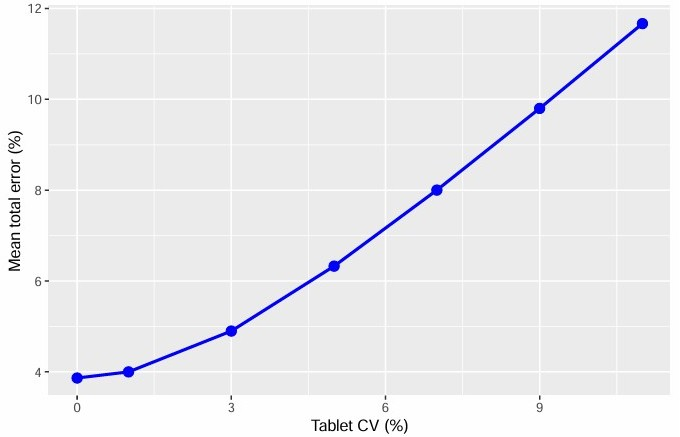
\includegraphics[width=0.8\textwidth]{Effect of tablet CV on total error}
\caption{\footnotesize Effect of tablet CV on total error. This graph illustrates how the mean total error of the FOVS concentration estimate changes when the tablet CV increases from 0\% to 11\%, while all other parameters remain constant.}
\label{fig:tablet-total-error}
\end{figure}

The corresponding numerical decomposition for scenario 1, including the
tablet, calibration, and marker counting error components, is provided
in Table \ref{tab:tablet-error-components}. Figure
\ref{fig:tablet-error-shares} presents the relative contributions of the
three error components to the total error.

(See ``Error decomposition across tablet CV levels'' and ``Code for
Figure 2'' in Appendix C.3 and C.4. The error components reported in
Table \ref{tab:tablet-error-components} were obtained from
\texttt{summary\_cv.csv} and formatted on lines 53--62 of
\texttt{analysis\_Fossil.R}. Their relative contributions were
calculated on lines 65--70, reshaped on lines 82--93, and plotted in
Figure \ref{fig:tablet-error-shares} on lines 95--102 of the same file.)

\begin{table}[ht!]
\centering
\small
\resizebox{\textwidth}{!}{
\begin{tabular}{rrrrr}
\hline
tablet\_cv &
mean\_tablet\_term(\%) &
mean\_calibration\_term(\%) &
mean\_marker\_term(\%) &
mean\_theoretical\_error(\%) \\
\hline
0.00 & 0  & 2.20 & 3.16 & 3.86  \\
0.01 & 1  & 2.21 & 3.16 & 4.00  \\
0.03 & 3  & 2.21 & 3.16 & 4.90  \\
0.05 & 5  & 2.21 & 3.17 & 6.33  \\
0.07 & 7  & 2.21 & 3.17 & 8.00  \\
0.09 & 9  & 2.20 & 3.17 & 9.80  \\
0.11 & 11 & 2.20 & 3.18 & 11.67 \\
\hline
\end{tabular}
}
\caption{\footnotesize Error decomposition across tablet CV levels. This table reports the tablet, calibration, and marker counting error components and the resulting mean theoretical total error for each CV.}
\label{tab:tablet-error-components}
\end{table}

\begin{figure}
\centering
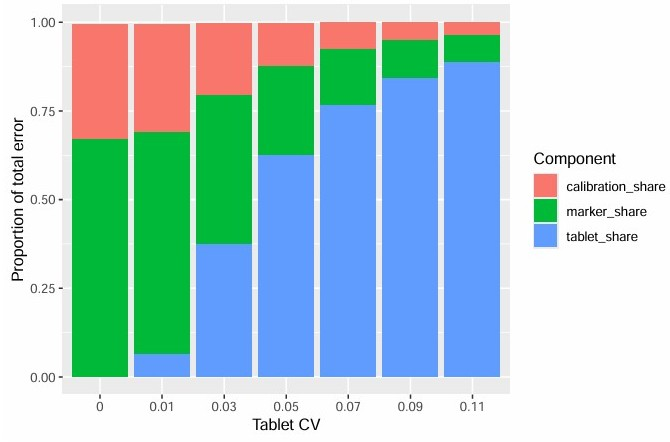
\includegraphics[width=0.8\textwidth]{relative contributions across tablet CV levels}
\caption{\footnotesize Relative contributions of error components across tablet CV levels. This graph illustrates the proportion of tablet, calibration and marker counting error in the total error as the tablet CV changes.}
\label{fig:tablet-error-shares}
\end{figure}

\subsection{Effect of tablet number on tablet and total
error}\label{effect-of-tablet-number-on-tablet-and-total-error}

The simulation outputs of scenario 2 are contained in Table
\ref{tab:n1-results}. The table reports the mean true concentration,
mean estimated concentration, mean theoretical total error, and mean
effort. The trend of the mean total error varying with N1 is plotted in
Figure \ref{fig:n1-total-error}.

(See ``N1 scenario code and output'' and ``Code for Figure 3'' in
Appendix D.1 and D.2. The values reported in Table \ref{tab:n1-results}
are contained in \texttt{summary\_N1.csv} and were selected and
formatted on lines 107--121 of \texttt{analysis\_Fossil.R}. Figure
\ref{fig:n1-total-error} was generated from the same results on lines
123--131 of the same file.)

\begin{table}[ht!]
\centering
\resizebox{\textwidth}{!}{
\begin{tabular}{rrrrrrr}
\hline
N1 &
tablet\_cv &
tablet\_mean &
mean\_true\_conc &
mean\_estimated\_conc &
mean\_theoretical\_error(\%) &
mean\_effort \\
\hline
1 & 0.04 & 5000.00 & 10000 & 10032.98 & 5.57 & 3078.21 \\
2 & 0.04 & 2500.00 & 10000 & 10016.91 & 4.80 & 3079.84 \\
4 & 0.04 & 1250.00 & 10000 & 10014.14 & 4.36 & 3079.77 \\
6 & 0.04 &  833.33 & 10000 & 10007.29 & 4.20 & 3079.42 \\
\hline
\end{tabular}
}
\caption{\footnotesize Simulation results across tablet number. This table summarizes the main indicators obtained from 5,000 repeated simulations for $N_1=1, 2, 4, 6$.}
\label{tab:n1-results}
\end{table}

\begin{figure}
\centering
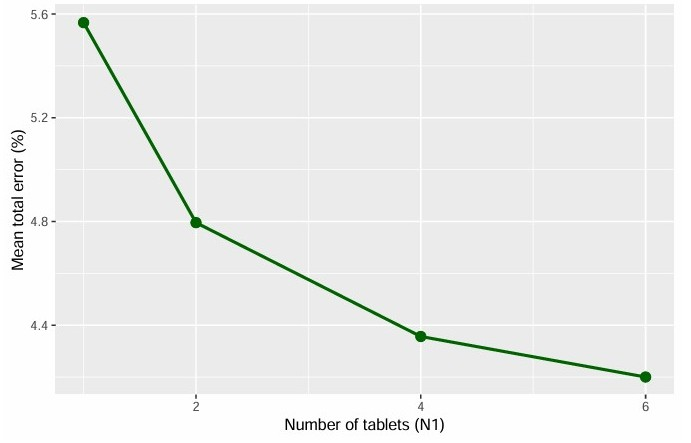
\includegraphics[width=0.8\textwidth]{Effect of N1 on total error}
\caption{\footnotesize Effect of number of tablets on total error. This graph illustrates how the mean total error of the FOVS concentration estimate changes when N1 increases, while all other parameters remain constant.}
\label{fig:n1-total-error}
\end{figure}

The numerical decomposition of the total error for scenario 2, including
the tablet, calibration, and marker counting components, is contained in
Table \ref{tab:n1-error-components}. The relative contributions of these
components are presented in Figure \ref{fig:n1-error-shares}.

(See ``Error decomposition across numbers of tablets'' and ``Code for
Figure 4'' in Appendix D.3 and D.4. The error components reported in
Table \ref{tab:n1-error-components} were obtained from
\texttt{summary\_N1.csv} and formatted on lines 133--142 of
\texttt{analysis\_Fossil.R}. Their relative contributions were
calculated on lines 144--149, reshaped on lines 161--172, and plotted in
Figure \ref{fig:n1-error-shares} on lines 174--181 of the same file.)

\begin{table}[ht!]
\centering
\resizebox{\textwidth}{!}{
\begin{tabular}{rrrrr}
\hline
N1 &
mean\_tablet\_term(\%) &
mean\_calibration\_term(\%) &
mean\_marker\_term(\%) &
mean\_theoretical\_error(\%) \\
\hline
1 & 4.00 & 2.20 & 3.17 & 5.57 \\
2 & 2.83 & 2.21 & 3.16 & 4.80 \\
4 & 2.00 & 2.21 & 3.16 & 4.36 \\
6 & 1.63 & 2.21 & 3.16 & 4.20 \\
\hline
\end{tabular}
}
\caption{\footnotesize Error decomposition across numbers of tablets. This table reports the tablet, calibration, and marker error components and the resulting mean theoretical total error for each $N_1$.}
\label{tab:n1-error-components}
\end{table}

\begin{figure}
\centering
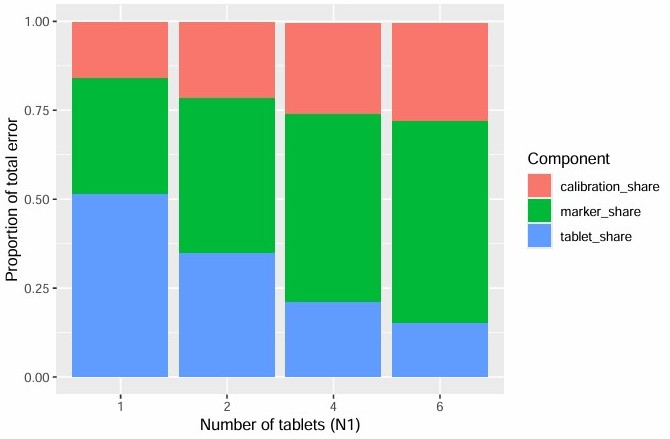
\includegraphics[width=0.8\textwidth]{relative contributions across N1}
\caption{\footnotesize Relative contributions of error components across numbers of tablets. This figure shows the proportion of tablet, calibration and marker counting error in the total error as $N_1$ varies.}
\label{fig:n1-error-shares}
\end{figure}

\subsection{Effect of target-to-marker ratio on the error
structure}\label{effect-of-target-to-marker-ratio-on-the-error-structure}

The simulation outputs of scenario 3 are contained in Table
\ref{tab:ratio-results}. The corresponding mean total errors across
target-to-marker ratio are plotted in Figure
\ref{fig:ratio-total-error}.

(See ``Target-to-marker ratio scenario code and output'' and ``Code for
Figure 5'' in Appendix E.1 and E.2. The values reported in Table
\ref{tab:ratio-results} are contained in \texttt{summary\_ratio.csv} and
were selected and formatted on lines 187--202 of
\texttt{analysis\_Fossil.R}. Figure \ref{fig:ratio-total-error} was
generated from the same results on lines 204--212 of
\texttt{analysis\_Fossil.R}.)

\begin{table}[ht!]
\centering
\resizebox{\textwidth}{!}{
\begin{tabular}{rrrrrrrrr}
\hline
ratio &
N1 &
tablet\_cv &
tablet\_mean &
mean\_true\_conc &
mean\_estimated\_conc &
mean\_theoretical\_error(\%) &
mean\_effort \\
\hline
1  & 1 & 0.04 & 10000.00 & 10000 & 10026.91 & 5.10 & 4078.43 \\
2  & 1 & 0.04 &  5000.00 & 10000 & 10018.62 & 5.57 & 3079.36 \\
4  & 1 & 0.04 &  2500.00 & 10000 & 10025.48 & 6.41 & 2579.89 \\
6  & 1 & 0.04 &  1666.67 & 10000 & 10038.58 & 7.15 & 2412.98 \\
8  & 1 & 0.04 &  1250.00 & 10000 & 10043.79 & 7.82 & 2330.57 \\
10 & 1 & 0.04 &  1000.00 & 10000 & 10068.92 & 8.44 & 2279.91 \\
15 & 1 & 0.04 &   666.67 & 10000 & 10090.61 & 9.83 & 2212.30 \\
\hline
\end{tabular}
}
\caption{\footnotesize Simulation results across target-to-marker ratio. This table summarizes the main indicators obtained from 5,000 repeated simulations for target-to-marker ratios of 1, 2, 4, 6, 8, 10, and 15.}
\label{tab:ratio-results}
\end{table}

\begin{figure}
\centering
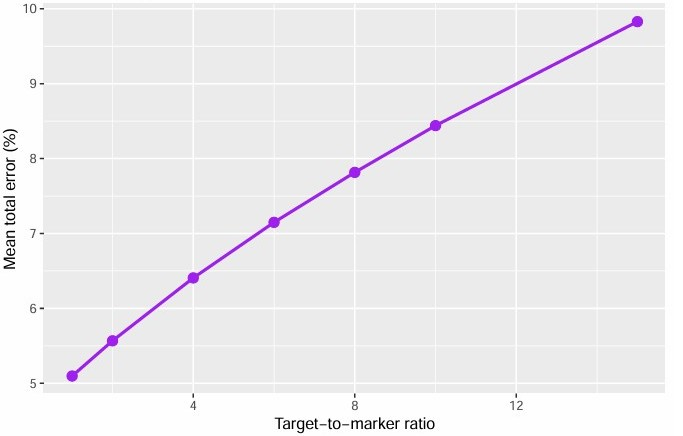
\includegraphics[width=0.8\textwidth]{Effect of target-to-marker ratio on total error}
\caption{\footnotesize Effect of target-to-marker ratio on total error. This graph illustrates how the mean total error of the FOVS concentration estimate changes when the target-to-marker ratio varies, while all other parameters remain constant.}
\label{fig:ratio-total-error}
\end{figure}

The numerical decomposition of the total error for scenario 3, including
tablet, calibration, and marker counting components, is contained in
Table \ref{tab:ratio-error-components}. The relative contributions of
these components are presented in Figure \ref{fig:ratio-error-shares}.

(See ``Error decomposition across ratio'' and ``Code for Figure 6'' in
Appendix E.3 and E.4. The error components reported in Table
\ref{tab:ratio-error-components} were obtained from
\texttt{summary\_ratio.csv} and formatted on lines 214--223 of
\texttt{analysis\_Fossil.R}. Their relative contributions were
calculated on lines 226--231, reshaped on lines 243--254, and plotted in
Figure \ref{fig:ratio-error-shares} on lines 256--263 of the same file.)

\begin{table}[ht!]
\centering
\resizebox{\textwidth}{!}{
\begin{tabular}{rrrrr}
\hline
ratio &
mean\_tablet\_term(\%) &
mean\_calibration\_term(\%) &
mean\_marker\_term(\%) &
mean\_theoretical\_error(\%) \\
\hline
1  & 4.00 & 2.21 & 2.24 & 5.10 \\
2  & 4.00 & 2.20 & 3.16 & 5.57 \\
4  & 4.00 & 2.21 & 4.48 & 6.41 \\
6  & 4.00 & 2.21 & 5.49 & 7.15 \\
8  & 4.00 & 2.20 & 6.33 & 7.82 \\
10 & 4.00 & 2.20 & 7.09 & 8.44 \\
15 & 4.00 & 2.21 & 8.69 & 9.83 \\
\hline
\end{tabular}
}
\caption{\footnotesize Error decomposition across target-to-marker ratio. This table reports the mean tablet, calibration, and marker error components and the resulting mean theoretical total error for each target-to-marker ratio level.}
\label{tab:ratio-error-components}
\end{table}

\begin{figure}
\centering
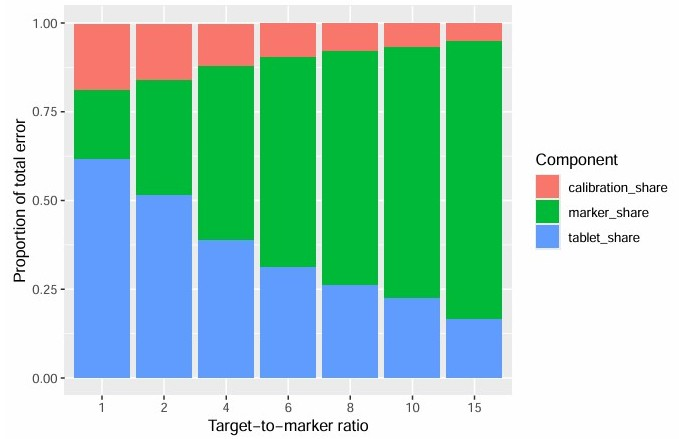
\includegraphics[width=0.8\textwidth]{relative contributions across ratio}
\caption{\footnotesize Relative contributions of error components across target-to-marker ratio. This figure shows the proportion of tablet, calibration and marker counting error in the total error as ratio varies.}
\label{fig:ratio-error-shares}
\end{figure}

\section{Discussion}\label{discussion}

\subsection{Tablet CV as a limitation on FOVS
precision}\label{tablet-cv-as-a-limitation-on-fovs-precision}

Table \ref{tab:tablet-cv-results} shows that when the tablet CV
increases from 0 to 0.11, the mean theoretical error rises from 3.86\%
to 11.67\%. We can also more intuitively observe this trend from Figure
\ref{fig:tablet-total-error}, which indicates that the tablet error
reduces the precision of the FOVS concentration estimates. Table
\ref{tab:tablet-error-components} further indicates that this increase
is mainly due to the tablet error term increasing from 0\% to 11.00\%,
while calibration and marker counting errors remain basically unchanged.
Therefore, even if the FOVS counting design is exactly the same, the
actual marker dose variation in the tablet may still make the final
estimate unreliable.

Figure \ref{fig:tablet-error-shares} shows that when the CV reaches
0.05, the tablet error accounts for approximately 62\% and has become
the main source of error; when the CV is 0.11, this proportion is close
to 90\%. This means that when the tablet CV is low, the precision can be
improved mainly by enhancing the markers and calibration counts.
However, when the CV is high, simply increasing the count quantity will
have very limited effect, because the main variation has already been
introduced by the tablet dose before the counting begins.

Furthermore, the mean estimated concentration shown in Table
\ref{tab:tablet-cv-results} also slightly increases as the CV increases,
which indicates that the tablet error may also cause a certain upward
shift in the average result. In conclusion, the increasing CV clearly
affects the final estimation precision, and this effect mainly stems
from the tablet error term.

\subsection{Using multiple tablets to reduce tablet
error}\label{using-multiple-tablets-to-reduce-tablet-error}

Figure \ref{fig:n1-total-error} shows that when \(N_1\) increases from 1
to 6, the mean theoretical error obviously decreases, from 5.57\% to
4.20\% (values from Table \ref{tab:n1-results}). According to Table
\ref{tab:n1-error-components}, the tablet error term decreases from
4.00\% to 1.63\%, while the calibration and marker counting errors
remain largely unchanged. This means that when dose variation among
tablets is independent, distributing the marker dose to more independent
tablets allows some of the random variation to cancel out, thereby
stabilizing the total marker dose.

In other words, if tablet errors have become a main source of errors,
then using multiple independent tablets might be more reliable than
relying on a single tablet. However, Figure \ref{fig:n1-error-shares}
shows that as tablet number increases, the contribution of tablet term
decreases, while marker counting errors gradually become the largest
source of error. Therefore, increasing the tablet number does indeed
effectively improve the estimation precision, but it is most helpful
only when the tablet error is relatively large. Once marker counting
error becomes dominant, further increasing the tablet number provides
only limited improvement. At this point, increasing the actual marker
count might be more effective.

\subsection{Target-to-marker ratio changes the importance of tablet
error}\label{target-to-marker-ratio-changes-the-importance-of-tablet-error}

Figure \ref{fig:ratio-total-error} shows that as the target-to-marker
ratio increases, the mean theoretical error substantially rises, from
5.10\% to 9.83\% (values from Table \ref{tab:ratio-results}). The main
factor causing this change is the marker counting error. As can be seen
from Table \ref{tab:ratio-error-components}, the tablet and calibration
errors remain relatively stable, but the marker counting error increases
from 2.24\% to 8.69\%.

Figure \ref{fig:ratio-error-shares} also shows that when ratio is 1 or
2, tablet error is the main source of errors. This means that when there
are already enough markers, adding more markers may not greatly improve
precision because tablet error becomes the main limitation. In this
case, using tablets with a lower CV or more independent tablets may be
more effective. However, as the ratio increases, the relative
contribution of tablet error decreases, which does not mean that tablet
error itself has been reduced. Instead, the larger marker counting error
caused by the fewer markers makes the effect of tablet error less
noticeable.

Furthermore, Table \ref{tab:ratio-results} also shows that when ratio is
1, mean theoretical error is the lowest; when ratio increases to 2, mean
theoretical error only increases from 5.10\% to 5.57\%, while mean
effort decreases from approximately 4,078 to 3,080. Therefore, a ratio
of 2 can be regarded as a reasonable balance between precision and
effort under the conditions of this study.

\subsection{Limitations and future
work}\label{limitations-and-future-work}

This study separately examines the independent effects of tablet CV,
tablet number, and target-to-marker ratio. However, in actual
experiments, these three factors usually change simultaneously and may
also influence each other. Subsequent studies can adopt a comprehensive
simulation design and simultaneously compare the different combinations
of the three factors, thereby testing whether there are any interactions
among them. For instance, the effect of increasing tablet number in
reducing tablet error might be more pronounced when the tablet CV is
relatively high; however, when the target-to-marker ratio is high and
marker counting error becomes the main source of errors, this
improvement might be relatively limited. By comparing the total
theoretical error, the three error components, and the effort under
different combinations, it is possible to further determine under which
conditions the tablet error is the most significant. Based on this, an
acceptable error level can be set, and the parameter combination
requiring the least effort to achieve the corresponding precision could
then be identified. This would provide more direct guidance for
selecting tablet number and marker dose in experimental design.

\section{Acknowledgements}\label{acknowledgements}

I would like to thank my project supervisor, Anthony Mays, for his
guidance and advice throughout this project. I also thank my group
members and classmates for helpful discussions, suggestions, and
assistance in clarifying some questions during the development of this
report. I acknowledge that the structure of this report was prepared
with reference to the Part B Report template provided for this course. I
acknowledge that I used ChatGPT to help me clarify the easily confused
terminology. The code, simulation outputs, and source files supporting
this report are available in the following public GitHub repository:
\url{https://github.com/FFMMHH-13/MDSresearch_FinalReport_-Fu-_-M-}.

\section{References}\label{references}

\phantomsection\label{refs}
\begin{CSLReferences}{1}{0}
\bibitem[\citeproctext]{ref-BenninghoffWS1962}
Benninghoff, W. S. 1962. {``Calculation of Pollen and Spore Density in
Sediments by Addition of Exotic Pollen in Known Quantities.''}
\emph{Pollen Et Spores} 4 (2): 332--33.

\bibitem[\citeproctext]{ref-JacksonDonaldA1997CDiC}
Jackson, Donald A. 1997. {``Compositional Data in Community Ecology: The
Paradigm or Peril of Proportions?''} \emph{Ecology (Durham)} 78 (3):
929--40.

\bibitem[\citeproctext]{ref-MaherLouisJ1981Sfmc}
Maher, Louis J. 1981. {``Statistics for Microfossil Concentration
Measurements Employing Samples Spiked with Marker Grains.''}
\emph{Review of Palaeobotany and Palynology} 32 (2): 153--91.

\bibitem[\citeproctext]{ref-MaysChris2025FsAn}
Mays, Chris, Marcos Amores, and Anthony Mays. 2025. {``Field-of-View
Subsampling: A Novel {`Exotic Marker'} Method for Absolute Abundances,
Validated by Simulation and Microfossil Case Studies.''} \emph{PloS One}
20 (5): e0320887--.

\bibitem[\citeproctext]{ref-PriceAndreaMichelle2016Dtaa}
Price, Andrea Michelle, Pieter Roger Gurdebeke, Kenneth Neil Mertens,
and Vera Pospelova. 2016. {``Determining the Absolute Abundance of
Dinoflagellate Cysts in Recent Marine Sediments III: Identifying the
Source of Lycopodium Loss During Palynological Processing and Further
Testing of the Lycopodium Marker-Grain Method.''} \emph{Review of
Palaeobotany and Palynology} 226: 78--90.

\bibitem[\citeproctext]{ref-stockmarr1973}
Stockmarr, J. 1973. {``Determination of Spore Concentration with an
Electronic Particle Counter.''} \emph{Geological Survey of Denmark
Yearbook 1972}, 87--89.

\bibitem[\citeproctext]{ref-stockmarr1971}
Stockmarr, J. 1971. {``Tablets with Spores Used in Absolute Pollen
Analysis.''} \emph{Pollen Et Spores} 13 (4): 615--21.

\end{CSLReferences}

\newpage

\section{Statistical appendix}\label{statistical-appendix}

\subsection{Appendix A: Core simulation
function}\label{appendix-a-core-simulation-function}

\subsubsection{Appendix A.1: Simulation settings and target
generation}\label{appendix-a.1-simulation-settings-and-target-generation}

This code defines the basic simulation settings and generates the target
particles within the two-dimensional sample region. (Supports Step 1 of
Section 5.1, the common simulation settings in Table 1, and Sections
6.1--6.3.)

\begin{Shaded}
\begin{Highlighting}[]
\NormalTok{simulate\_fovs\_once }\OtherTok{\textless{}{-}} \ControlFlowTok{function}\NormalTok{(}
  \AttributeTok{n\_target =} \DecValTok{10000}\NormalTok{,}
  \AttributeTok{N1 =} \DecValTok{1}\NormalTok{,}
  \AttributeTok{tablet\_mean =} \DecValTok{5000}\NormalTok{,}
  \AttributeTok{tablet\_cv =} \DecValTok{0}\NormalTok{,}
  \AttributeTok{region\_side =} \DecValTok{1}\NormalTok{,}
  \AttributeTok{fov\_size =} \FloatTok{0.1}\NormalTok{,}
  \AttributeTok{n\_cal =} \DecValTok{20}\NormalTok{,}
  \AttributeTok{n\_ext =} \DecValTok{20}\NormalTok{,}
  \AttributeTok{omega =} \DecValTok{2}
\NormalTok{) \{}
  
  \CommentTok{\# Sample area}
\NormalTok{  V }\OtherTok{\textless{}{-}}\NormalTok{ region\_side}\SpecialCharTok{\^{}}\DecValTok{2}
  \CommentTok{\# True concentration}
\NormalTok{  true\_conc }\OtherTok{\textless{}{-}}\NormalTok{ n\_target }\SpecialCharTok{/}\NormalTok{ V}
  \CommentTok{\# Generate target particles}
\NormalTok{  points }\OtherTok{\textless{}{-}} \FunctionTok{tibble}\NormalTok{(}
    \AttributeTok{x =} \FunctionTok{runif}\NormalTok{(n\_target, }\AttributeTok{min =} \DecValTok{0}\NormalTok{, }\AttributeTok{max =}\NormalTok{ region\_side),}
    \AttributeTok{y =} \FunctionTok{runif}\NormalTok{(n\_target, }\AttributeTok{min =} \DecValTok{0}\NormalTok{, }\AttributeTok{max =}\NormalTok{ region\_side)}
\NormalTok{  )}
\end{Highlighting}
\end{Shaded}

\subsubsection{Appendix A.2: Tablet dose variation and marker
generation}\label{appendix-a.2-tablet-dose-variation-and-marker-generation}

This code generates the marker particles and introduces tablet dose
variation by simulating random marker doses for individual tablets.
(Supports Steps 2 and 3 of Section 5.1, the tablet-dose simulation used
in Sections 5.2--5.4, and Sections 6.1--6.3.)

\begin{Shaded}
\begin{Highlighting}[]
  \CommentTok{\# Known average marker dose used in the estimator}
\NormalTok{  known\_marker\_dose }\OtherTok{\textless{}{-}}\NormalTok{ N1 }\SpecialCharTok{*}\NormalTok{ tablet\_mean}
  \CommentTok{\# Generate per{-}tablet marker doses, then sum them}
\NormalTok{  tablet\_sd }\OtherTok{\textless{}{-}}\NormalTok{ tablet\_mean }\SpecialCharTok{*}\NormalTok{ tablet\_cv}
\NormalTok{  tablet\_doses }\OtherTok{\textless{}{-}} \FunctionTok{rnorm}\NormalTok{(N1, }\AttributeTok{mean =}\NormalTok{ tablet\_mean, }\AttributeTok{sd =}\NormalTok{ tablet\_sd)}
\NormalTok{  tablet\_doses }\OtherTok{\textless{}{-}} \FunctionTok{pmax}\NormalTok{(}\FunctionTok{round}\NormalTok{(tablet\_doses), }\DecValTok{1}\NormalTok{)}
\NormalTok{  true\_marker\_total }\OtherTok{\textless{}{-}} \FunctionTok{sum}\NormalTok{(tablet\_doses)}
  \CommentTok{\# Generate marker particles}
\NormalTok{  markers }\OtherTok{\textless{}{-}} \FunctionTok{tibble}\NormalTok{(}
    \AttributeTok{x =} \FunctionTok{runif}\NormalTok{(true\_marker\_total, }\AttributeTok{min =} \DecValTok{0}\NormalTok{, }\AttributeTok{max =}\NormalTok{ region\_side),}
    \AttributeTok{y =} \FunctionTok{runif}\NormalTok{(true\_marker\_total, }\AttributeTok{min =} \DecValTok{0}\NormalTok{, }\AttributeTok{max =}\NormalTok{ region\_side)}
\NormalTok{  )}
\end{Highlighting}
\end{Shaded}

\subsubsection{Appendix A.3: FOV grid construction and sampling
design}\label{appendix-a.3-fov-grid-construction-and-sampling-design}

This code constructs the FOV grid and selects calibration and
extrapolation FOVs from a shared local region. (Supports Step 4 of
Section 5.1 and the FOV sampling design used in Sections 6.1--6.3.)

\begin{Shaded}
\begin{Highlighting}[]
  \CommentTok{\# Build grid of candidate FOV locations}
\NormalTok{  n\_side }\OtherTok{\textless{}{-}}\NormalTok{ region\_side }\SpecialCharTok{/}\NormalTok{ fov\_size}
  \ControlFlowTok{if}\NormalTok{ (}\FunctionTok{abs}\NormalTok{(n\_side }\SpecialCharTok{{-}} \FunctionTok{round}\NormalTok{(n\_side)) }\SpecialCharTok{\textgreater{}} \FloatTok{1e{-}10}\NormalTok{) \{}
    \FunctionTok{stop}\NormalTok{(}\StringTok{"fov\_size must divide the region side exactly."}\NormalTok{)}
\NormalTok{  \}}

\NormalTok{  all\_grid }\OtherTok{\textless{}{-}} \FunctionTok{expand.grid}\NormalTok{(}
    \AttributeTok{x =} \FunctionTok{seq}\NormalTok{(}\DecValTok{0}\NormalTok{, region\_side }\SpecialCharTok{{-}}\NormalTok{ fov\_size, }\AttributeTok{by =}\NormalTok{ fov\_size),}
    \AttributeTok{y =} \FunctionTok{seq}\NormalTok{(}\DecValTok{0}\NormalTok{, region\_side }\SpecialCharTok{{-}}\NormalTok{ fov\_size, }\AttributeTok{by =}\NormalTok{ fov\_size)}
\NormalTok{  )}

  \CommentTok{\# Remove outermost edge cells}
\NormalTok{  inner\_grid }\OtherTok{\textless{}{-}} \FunctionTok{subset}\NormalTok{(}
\NormalTok{    all\_grid,}
\NormalTok{    x }\SpecialCharTok{\textgreater{}} \DecValTok{0} \SpecialCharTok{\&}\NormalTok{ x }\SpecialCharTok{\textless{}}\NormalTok{ (region\_side }\SpecialCharTok{{-}}\NormalTok{ fov\_size) }\SpecialCharTok{\&}
\NormalTok{    y }\SpecialCharTok{\textgreater{}} \DecValTok{0} \SpecialCharTok{\&}\NormalTok{ y }\SpecialCharTok{\textless{}}\NormalTok{ (region\_side }\SpecialCharTok{{-}}\NormalTok{ fov\_size)}
\NormalTok{  )}

  \ControlFlowTok{if}\NormalTok{ (}\FunctionTok{nrow}\NormalTok{(inner\_grid) }\SpecialCharTok{\textless{}}\NormalTok{ n\_cal }\SpecialCharTok{+}\NormalTok{ n\_ext) \{}
    \FunctionTok{stop}\NormalTok{(}\StringTok{"Not enough inner grid cells for the requested number of FOVs."}\NormalTok{)}
\NormalTok{  \}}

  \CommentTok{\# Define a shared local window so calibration and }
  \CommentTok{\# extrapolation FOVs come from nearby locations}
\NormalTok{  window\_cols }\OtherTok{\textless{}{-}} \DecValTok{7}
\NormalTok{  window\_rows }\OtherTok{\textless{}{-}} \DecValTok{6}

\NormalTok{  x\_vals }\OtherTok{\textless{}{-}} \FunctionTok{sort}\NormalTok{(}\FunctionTok{unique}\NormalTok{(inner\_grid}\SpecialCharTok{$}\NormalTok{x))}
\NormalTok{  y\_vals }\OtherTok{\textless{}{-}} \FunctionTok{sort}\NormalTok{(}\FunctionTok{unique}\NormalTok{(inner\_grid}\SpecialCharTok{$}\NormalTok{y))}
\NormalTok{  inner\_nx }\OtherTok{\textless{}{-}} \FunctionTok{length}\NormalTok{(x\_vals)}
\NormalTok{  inner\_ny }\OtherTok{\textless{}{-}} \FunctionTok{length}\NormalTok{(y\_vals)}

  \ControlFlowTok{if}\NormalTok{ (window\_cols }\SpecialCharTok{\textgreater{}}\NormalTok{ inner\_nx }\SpecialCharTok{||}\NormalTok{ window\_rows }\SpecialCharTok{\textgreater{}}\NormalTok{ inner\_ny) \{}
    \FunctionTok{stop}\NormalTok{(}\StringTok{"Shared FOV window is too large for the inner grid."}\NormalTok{)}
\NormalTok{  \}}

\NormalTok{  start\_col }\OtherTok{\textless{}{-}} \FunctionTok{sample}\NormalTok{(}\DecValTok{1}\SpecialCharTok{:}\NormalTok{(inner\_nx }\SpecialCharTok{{-}}\NormalTok{ window\_cols }\SpecialCharTok{+} \DecValTok{1}\NormalTok{), }\AttributeTok{size =} \DecValTok{1}\NormalTok{)}
\NormalTok{  start\_row }\OtherTok{\textless{}{-}} \FunctionTok{sample}\NormalTok{(}\DecValTok{1}\SpecialCharTok{:}\NormalTok{(inner\_ny }\SpecialCharTok{{-}}\NormalTok{ window\_rows }\SpecialCharTok{+} \DecValTok{1}\NormalTok{), }\AttributeTok{size =} \DecValTok{1}\NormalTok{)}

\NormalTok{  window\_x }\OtherTok{\textless{}{-}}\NormalTok{ x\_vals[start\_col}\SpecialCharTok{:}\NormalTok{(start\_col }\SpecialCharTok{+}\NormalTok{ window\_cols }\SpecialCharTok{{-}} \DecValTok{1}\NormalTok{)]}
\NormalTok{  window\_y }\OtherTok{\textless{}{-}}\NormalTok{ y\_vals[start\_row}\SpecialCharTok{:}\NormalTok{(start\_row }\SpecialCharTok{+}\NormalTok{ window\_rows }\SpecialCharTok{{-}} \DecValTok{1}\NormalTok{)]}

\NormalTok{  shared\_grid }\OtherTok{\textless{}{-}} \FunctionTok{subset}\NormalTok{(}
\NormalTok{    inner\_grid,}
\NormalTok{    x }\SpecialCharTok{\%in\%}\NormalTok{ window\_x }\SpecialCharTok{\&}\NormalTok{ y }\SpecialCharTok{\%in\%}\NormalTok{ window\_y}
\NormalTok{  )}

  \ControlFlowTok{if}\NormalTok{ (}\FunctionTok{nrow}\NormalTok{(shared\_grid) }\SpecialCharTok{\textless{}}\NormalTok{ n\_cal }\SpecialCharTok{+}\NormalTok{ n\_ext) \{}
    \FunctionTok{stop}\NormalTok{(}\StringTok{"Not enough cells in the shared local FOV region."}\NormalTok{)}
\NormalTok{  \}}

  \CommentTok{\# Select calibration and extrapolation FOVs from the same local region}
\NormalTok{  cal\_idx }\OtherTok{\textless{}{-}} \FunctionTok{sample}\NormalTok{(}\DecValTok{1}\SpecialCharTok{:}\FunctionTok{nrow}\NormalTok{(shared\_grid), }\AttributeTok{size =}\NormalTok{ n\_cal, }\AttributeTok{replace =} \ConstantTok{FALSE}\NormalTok{)}
\NormalTok{  cal\_fovs }\OtherTok{\textless{}{-}}\NormalTok{ shared\_grid[cal\_idx, ]}

\NormalTok{  remaining\_grid }\OtherTok{\textless{}{-}}\NormalTok{ shared\_grid[}\SpecialCharTok{{-}}\NormalTok{cal\_idx, ]}
\NormalTok{  ext\_idx }\OtherTok{\textless{}{-}} \FunctionTok{sample}\NormalTok{(}\DecValTok{1}\SpecialCharTok{:}\FunctionTok{nrow}\NormalTok{(remaining\_grid), }\AttributeTok{size =}\NormalTok{ n\_ext, }\AttributeTok{replace =} \ConstantTok{FALSE}\NormalTok{)}
\NormalTok{  ext\_fovs }\OtherTok{\textless{}{-}}\NormalTok{ remaining\_grid[ext\_idx, ]}
\end{Highlighting}
\end{Shaded}

\subsubsection{Appendix A.4: Target and marker
counting}\label{appendix-a.4-target-and-marker-counting}

This code counts target particles in calibration FOVs and marker
particles in extrapolation FOVs. (Supports Steps 5 and 6 of Section 5.1
and the target and marker counts used in Sections 6.1--6.3.)

\begin{Shaded}
\begin{Highlighting}[]
  \CommentTok{\# Count fossils in calibration FOVs}
\NormalTok{  cal\_fossil }\OtherTok{\textless{}{-}} \FunctionTok{numeric}\NormalTok{(n\_cal)}
  \ControlFlowTok{for}\NormalTok{ (i }\ControlFlowTok{in} \DecValTok{1}\SpecialCharTok{:}\NormalTok{n\_cal) \{}
\NormalTok{    cal\_fossil[i] }\OtherTok{\textless{}{-}} \FunctionTok{sum}\NormalTok{(}
\NormalTok{      points}\SpecialCharTok{$}\NormalTok{x }\SpecialCharTok{\textgreater{}=}\NormalTok{ cal\_fovs}\SpecialCharTok{$}\NormalTok{x[i] }\SpecialCharTok{\&}
\NormalTok{      points}\SpecialCharTok{$}\NormalTok{x }\SpecialCharTok{\textless{}}\NormalTok{  cal\_fovs}\SpecialCharTok{$}\NormalTok{x[i] }\SpecialCharTok{+}\NormalTok{ fov\_size }\SpecialCharTok{\&}
\NormalTok{      points}\SpecialCharTok{$}\NormalTok{y }\SpecialCharTok{\textgreater{}=}\NormalTok{ cal\_fovs}\SpecialCharTok{$}\NormalTok{y[i] }\SpecialCharTok{\&}
\NormalTok{      points}\SpecialCharTok{$}\NormalTok{y }\SpecialCharTok{\textless{}}\NormalTok{  cal\_fovs}\SpecialCharTok{$}\NormalTok{y[i] }\SpecialCharTok{+}\NormalTok{ fov\_size}
\NormalTok{    )}
\NormalTok{  \}}

  \CommentTok{\# Count markers in extrapolation FOVs}
\NormalTok{  ext\_marker }\OtherTok{\textless{}{-}} \FunctionTok{numeric}\NormalTok{(n\_ext)}
  \ControlFlowTok{for}\NormalTok{ (i }\ControlFlowTok{in} \DecValTok{1}\SpecialCharTok{:}\NormalTok{n\_ext) \{}
\NormalTok{    ext\_marker[i] }\OtherTok{\textless{}{-}} \FunctionTok{sum}\NormalTok{(}
\NormalTok{      markers}\SpecialCharTok{$}\NormalTok{x }\SpecialCharTok{\textgreater{}=}\NormalTok{ ext\_fovs}\SpecialCharTok{$}\NormalTok{x[i] }\SpecialCharTok{\&}
\NormalTok{      markers}\SpecialCharTok{$}\NormalTok{x }\SpecialCharTok{\textless{}}\NormalTok{  ext\_fovs}\SpecialCharTok{$}\NormalTok{x[i] }\SpecialCharTok{+}\NormalTok{ fov\_size }\SpecialCharTok{\&}
\NormalTok{      markers}\SpecialCharTok{$}\NormalTok{y }\SpecialCharTok{\textgreater{}=}\NormalTok{ ext\_fovs}\SpecialCharTok{$}\NormalTok{y[i] }\SpecialCharTok{\&}
\NormalTok{      markers}\SpecialCharTok{$}\NormalTok{y }\SpecialCharTok{\textless{}}\NormalTok{  ext\_fovs}\SpecialCharTok{$}\NormalTok{y[i] }\SpecialCharTok{+}\NormalTok{ fov\_size}
\NormalTok{    )}
\NormalTok{  \}}
\end{Highlighting}
\end{Shaded}

\subsubsection{Appendix A.5: Concentration, effort, and error
calculation}\label{appendix-a.5-concentration-effort-and-error-calculation}

This code calculates effort, the concentration estimate, and the three
components of theoretical total error. (Supports Step 7 of Section 5.1,
Sections 5.5.1 and 5.5.2, and the concentration, effort, and error
results reported in Sections 6.1--6.3.)

\begin{Shaded}
\begin{Highlighting}[]
  \CommentTok{\# Calculate effort}
\NormalTok{  x\_total }\OtherTok{\textless{}{-}} \FunctionTok{sum}\NormalTok{(cal\_fossil)}
\NormalTok{  n\_count }\OtherTok{\textless{}{-}} \FunctionTok{sum}\NormalTok{(ext\_marker)}
\NormalTok{  effort }\OtherTok{\textless{}{-}}\NormalTok{ (omega }\SpecialCharTok{*}\NormalTok{ n\_cal) }\SpecialCharTok{+}\NormalTok{ x\_total }\SpecialCharTok{+}\NormalTok{ (omega }\SpecialCharTok{*}\NormalTok{ n\_ext) }\SpecialCharTok{+}\NormalTok{ n\_count}

  \CommentTok{\# Calculate concentration and error}
\NormalTok{  ybar }\OtherTok{\textless{}{-}} \FunctionTok{mean}\NormalTok{(cal\_fossil)}
\NormalTok{  xhat }\OtherTok{\textless{}{-}}\NormalTok{ ybar }\SpecialCharTok{*}\NormalTok{ n\_ext}

\NormalTok{  failed }\OtherTok{\textless{}{-}}\NormalTok{ (n\_count }\SpecialCharTok{==} \DecValTok{0} \SpecialCharTok{||}\NormalTok{ ybar }\SpecialCharTok{==} \DecValTok{0}\NormalTok{)}

  \ControlFlowTok{if}\NormalTok{ (failed) \{}
\NormalTok{    conc }\OtherTok{\textless{}{-}} \ConstantTok{NA}
\NormalTok{    tablet\_term }\OtherTok{\textless{}{-}} \ConstantTok{NA}
\NormalTok{    calibration\_term }\OtherTok{\textless{}{-}} \ConstantTok{NA}
\NormalTok{    marker\_term }\OtherTok{\textless{}{-}} \ConstantTok{NA}
\NormalTok{    total\_error }\OtherTok{\textless{}{-}} \ConstantTok{NA}
\NormalTok{    bias }\OtherTok{\textless{}{-}} \ConstantTok{NA}
\NormalTok{    percent\_bias }\OtherTok{\textless{}{-}} \ConstantTok{NA}
\NormalTok{    s3p }\OtherTok{\textless{}{-}} \ConstantTok{NA}
\NormalTok{  \} }\ControlFlowTok{else}\NormalTok{ \{}
\NormalTok{    conc }\OtherTok{\textless{}{-}}\NormalTok{ (xhat }\SpecialCharTok{*}\NormalTok{ known\_marker\_dose) }\SpecialCharTok{/}\NormalTok{ (n\_count }\SpecialCharTok{*}\NormalTok{ V)}
\NormalTok{    s3p }\OtherTok{\textless{}{-}} \FunctionTok{sd}\NormalTok{(cal\_fossil) }\SpecialCharTok{/} \FunctionTok{mean}\NormalTok{(cal\_fossil)}

    \CommentTok{\# Error decomposition}
\NormalTok{    tablet\_term }\OtherTok{\textless{}{-}} \DecValTok{100} \SpecialCharTok{*}\NormalTok{ (tablet\_cv }\SpecialCharTok{/} \FunctionTok{sqrt}\NormalTok{(N1))}
\NormalTok{    calibration\_term }\OtherTok{\textless{}{-}} \DecValTok{100} \SpecialCharTok{*}\NormalTok{ (s3p }\SpecialCharTok{/} \FunctionTok{sqrt}\NormalTok{(n\_cal))}
\NormalTok{    marker\_term }\OtherTok{\textless{}{-}} \DecValTok{100} \SpecialCharTok{*}\NormalTok{ (}\FunctionTok{sqrt}\NormalTok{(n\_count) }\SpecialCharTok{/}\NormalTok{ n\_count)}

\NormalTok{    total\_error }\OtherTok{\textless{}{-}} \FunctionTok{sqrt}\NormalTok{(}
\NormalTok{      tablet\_term}\SpecialCharTok{\^{}}\DecValTok{2} \SpecialCharTok{+}
\NormalTok{      calibration\_term}\SpecialCharTok{\^{}}\DecValTok{2} \SpecialCharTok{+}
\NormalTok{      marker\_term}\SpecialCharTok{\^{}}\DecValTok{2}
\NormalTok{    )}
\NormalTok{  \}}
\end{Highlighting}
\end{Shaded}

\subsection{Appendix B: Repeated simulation and summary
output}\label{appendix-b-repeated-simulation-and-summary-output}

\subsubsection{Appendix B.1: Repeated
simulations}\label{appendix-b.1-repeated-simulations}

This code repeatedly runs the core simulation and combines the outputs
into a single data set. (Supports Step 8 of Section 5.1 and the repeated
simulations reported in Sections 6.1--6.3.)

\begin{Shaded}
\begin{Highlighting}[]
\NormalTok{simulate\_fovs\_repeated }\OtherTok{\textless{}{-}} \ControlFlowTok{function}\NormalTok{(}
  \AttributeTok{n\_rep =} \DecValTok{5000}\NormalTok{,}
  \AttributeTok{n\_target =} \DecValTok{10000}\NormalTok{,}
  \AttributeTok{N1 =} \DecValTok{1}\NormalTok{,}
  \AttributeTok{tablet\_mean =} \DecValTok{5000}\NormalTok{,}
  \AttributeTok{tablet\_cv =} \DecValTok{0}\NormalTok{,}
  \AttributeTok{region\_side =} \DecValTok{1}\NormalTok{,}
  \AttributeTok{fov\_size =} \FloatTok{0.1}\NormalTok{,}
  \AttributeTok{n\_cal =} \DecValTok{20}\NormalTok{,}
  \AttributeTok{n\_ext =} \DecValTok{20}\NormalTok{,}
  \AttributeTok{omega =} \DecValTok{2}
\NormalTok{) \{}
\NormalTok{  results }\OtherTok{\textless{}{-}} \FunctionTok{vector}\NormalTok{(}\StringTok{"list"}\NormalTok{, n\_rep)}

  \ControlFlowTok{for}\NormalTok{ (k }\ControlFlowTok{in} \DecValTok{1}\SpecialCharTok{:}\NormalTok{n\_rep) \{}
\NormalTok{    results[[k]] }\OtherTok{\textless{}{-}} \FunctionTok{simulate\_fovs\_once}\NormalTok{(}
      \AttributeTok{n\_target =}\NormalTok{ n\_target,}
      \AttributeTok{N1 =}\NormalTok{ N1,}
      \AttributeTok{tablet\_mean =}\NormalTok{ tablet\_mean,}
      \AttributeTok{tablet\_cv =}\NormalTok{ tablet\_cv,}
      \AttributeTok{region\_side =}\NormalTok{ region\_side,}
      \AttributeTok{fov\_size =}\NormalTok{ fov\_size,}
      \AttributeTok{n\_cal =}\NormalTok{ n\_cal,}
      \AttributeTok{n\_ext =}\NormalTok{ n\_ext,}
      \AttributeTok{omega =}\NormalTok{ omega}
\NormalTok{    )}
\NormalTok{  \}}

\NormalTok{  results\_df }\OtherTok{\textless{}{-}} \FunctionTok{bind\_rows}\NormalTok{(results)}
\end{Highlighting}
\end{Shaded}

\subsubsection{Appendix B.2: Summary output
metrics}\label{appendix-b.2-summary-output-metrics}

This code calculates the summary statistics used in the report,
including mean true concentration, mean estimated concentration, mean
theoretical error and mean effort. (Supports Sections 5.5.1 and 5.5.2
and the summary statistics reported in Tables 2--7.)

\begin{Shaded}
\begin{Highlighting}[]
\NormalTok{  mean\_conc }\OtherTok{\textless{}{-}} \FunctionTok{mean}\NormalTok{(results\_df}\SpecialCharTok{$}\NormalTok{conc, }\AttributeTok{na.rm =} \ConstantTok{TRUE}\NormalTok{)}
\NormalTok{  sd\_conc }\OtherTok{\textless{}{-}} \FunctionTok{sd}\NormalTok{(results\_df}\SpecialCharTok{$}\NormalTok{conc, }\AttributeTok{na.rm =} \ConstantTok{TRUE}\NormalTok{)}
\NormalTok{  mean\_error }\OtherTok{\textless{}{-}} \FunctionTok{mean}\NormalTok{(results\_df}\SpecialCharTok{$}\NormalTok{total\_error, }\AttributeTok{na.rm =} \ConstantTok{TRUE}\NormalTok{)}
\NormalTok{  sim\_cv }\OtherTok{\textless{}{-}} \DecValTok{100} \SpecialCharTok{*}\NormalTok{ sd\_conc }\SpecialCharTok{/}\NormalTok{ mean\_conc}
  
\NormalTok{  summary\_df }\OtherTok{\textless{}{-}} \FunctionTok{tibble}\NormalTok{(}
    \AttributeTok{N1 =}\NormalTok{ N1,}
    \AttributeTok{tablet\_cv =}\NormalTok{ tablet\_cv,}
    \AttributeTok{mean\_true\_conc =} \FunctionTok{mean}\NormalTok{(results\_df}\SpecialCharTok{$}\NormalTok{true\_conc, }\AttributeTok{na.rm =} \ConstantTok{TRUE}\NormalTok{),}
    \AttributeTok{mean\_estimated\_conc =}\NormalTok{ mean\_conc,}
    \AttributeTok{empirical\_sd =}\NormalTok{ sd\_conc,}
    \AttributeTok{empirical\_cv =}\NormalTok{ sim\_cv,}
    \AttributeTok{mean\_tablet\_term =} \FunctionTok{mean}\NormalTok{(results\_df}\SpecialCharTok{$}\NormalTok{tablet\_term, }\AttributeTok{na.rm =} \ConstantTok{TRUE}\NormalTok{),}
     \AttributeTok{mean\_calibration\_term =} \FunctionTok{mean}\NormalTok{(results\_df}\SpecialCharTok{$}\NormalTok{calibration\_term, }\AttributeTok{na.rm =} \ConstantTok{TRUE}\NormalTok{),}
    \AttributeTok{mean\_marker\_term =} \FunctionTok{mean}\NormalTok{(results\_df}\SpecialCharTok{$}\NormalTok{marker\_term, }\AttributeTok{na.rm =} \ConstantTok{TRUE}\NormalTok{),}
    \AttributeTok{mean\_theoretical\_error =}\NormalTok{ mean\_error,}
    \AttributeTok{mean\_bias =} \FunctionTok{mean}\NormalTok{(results\_df}\SpecialCharTok{$}\NormalTok{bias, }\AttributeTok{na.rm =} \ConstantTok{TRUE}\NormalTok{),}
    \AttributeTok{mean\_percent\_bias =} \FunctionTok{mean}\NormalTok{(results\_df}\SpecialCharTok{$}\NormalTok{percent\_bias, }\AttributeTok{na.rm =} \ConstantTok{TRUE}\NormalTok{),}
    \AttributeTok{mean\_effort =} \FunctionTok{mean}\NormalTok{(results\_df}\SpecialCharTok{$}\NormalTok{effort, }\AttributeTok{na.rm =} \ConstantTok{TRUE}\NormalTok{),}
\NormalTok{  )}
\end{Highlighting}
\end{Shaded}

\subsection{Appendix C: Scenario 1
results}\label{appendix-c-scenario-1-results}

\subsubsection{Appendix C.1: Tablet CV scenario code and
output}\label{appendix-c.1-tablet-cv-scenario-code-and-output}

This code runs the repeated simulations across different tablet CV
levels and produces the corresponding summary results. (Supports the
Scenario 1 settings in Section 5.2 and Table 1, and the simulation
outputs reported in Section 6.1.)

\begin{Shaded}
\begin{Highlighting}[]
\FunctionTok{set.seed}\NormalTok{(}\DecValTok{456}\NormalTok{)}
\NormalTok{tablet\_cv\_levels }\OtherTok{\textless{}{-}} \FunctionTok{c}\NormalTok{(}\DecValTok{0}\NormalTok{, }\FloatTok{0.01}\NormalTok{, }\FloatTok{0.03}\NormalTok{, }\FloatTok{0.05}\NormalTok{, }\FloatTok{0.07}\NormalTok{, }\FloatTok{0.09}\NormalTok{, }\FloatTok{0.11}\NormalTok{)}

\NormalTok{results\_cv }\OtherTok{\textless{}{-}} \FunctionTok{vector}\NormalTok{(}\StringTok{"list"}\NormalTok{, }\FunctionTok{length}\NormalTok{(tablet\_cv\_levels))}

\ControlFlowTok{for}\NormalTok{ (i }\ControlFlowTok{in} \FunctionTok{seq\_along}\NormalTok{(tablet\_cv\_levels)) \{}
\NormalTok{  results\_cv[[i]] }\OtherTok{\textless{}{-}} \FunctionTok{simulate\_fovs\_repeated}\NormalTok{(}
    \AttributeTok{n\_rep =} \DecValTok{5000}\NormalTok{,}
    \AttributeTok{n\_target =} \DecValTok{10000}\NormalTok{,}
    \AttributeTok{N1 =} \DecValTok{1}\NormalTok{,}
    \AttributeTok{tablet\_mean =} \DecValTok{5000}\NormalTok{,}
    \AttributeTok{tablet\_cv =}\NormalTok{ tablet\_cv\_levels[i],}
    \AttributeTok{region\_side =} \DecValTok{1}\NormalTok{,}
    \AttributeTok{fov\_size =} \FloatTok{0.1}\NormalTok{,}
    \AttributeTok{n\_cal =} \DecValTok{20}\NormalTok{,}
    \AttributeTok{n\_ext =} \DecValTok{20}\NormalTok{,}
    \AttributeTok{omega =} \DecValTok{2}
\NormalTok{  )}\SpecialCharTok{$}\NormalTok{summary}
\NormalTok{\}}

\NormalTok{summary\_cv }\OtherTok{\textless{}{-}} \FunctionTok{bind\_rows}\NormalTok{(results\_cv)}
\end{Highlighting}
\end{Shaded}

\subsubsection{Appendix C.2: Code for Figure
1}\label{appendix-c.2-code-for-figure-1}

This code generates the figure showing the relationship between tablet
CV and mean total error. (Supports Figure 1 in Section 6.1.)

\begin{Shaded}
\begin{Highlighting}[]
\FunctionTok{ggplot}\NormalTok{(summary\_cv, }\FunctionTok{aes}\NormalTok{(}\AttributeTok{x =}\NormalTok{ tablet\_cv }\SpecialCharTok{*} \DecValTok{100}\NormalTok{, }\AttributeTok{y =}\NormalTok{ mean\_theoretical\_error)) }\SpecialCharTok{+}
  \FunctionTok{geom\_line}\NormalTok{(}\AttributeTok{linewidth =} \DecValTok{1}\NormalTok{, }\AttributeTok{colour =} \StringTok{"blue"}\NormalTok{) }\SpecialCharTok{+}
  \FunctionTok{geom\_point}\NormalTok{(}\AttributeTok{size =} \DecValTok{3}\NormalTok{, }\AttributeTok{colour =} \StringTok{"blue"}\NormalTok{) }\SpecialCharTok{+}
  \FunctionTok{labs}\NormalTok{(}
    \AttributeTok{title =} \StringTok{"Effect of tablet CV on total error"}\NormalTok{,}
    \AttributeTok{x =} \StringTok{"Tablet CV (\%)"}\NormalTok{,}
    \AttributeTok{y =} \StringTok{"Mean total error (\%)"}
\NormalTok{  )}
\end{Highlighting}
\end{Shaded}

\subsubsection{Appendix C.3: Error decomposition across tablet CV
levels}\label{appendix-c.3-error-decomposition-across-tablet-cv-levels}

This code extracts the three error components for the tablet CV
scenario. (Supports Table 3 in Section 6.1.)

\begin{Shaded}
\begin{Highlighting}[]
\NormalTok{summary\_cv }\SpecialCharTok{\%\textgreater{}\%}
  \FunctionTok{select}\NormalTok{(}
\NormalTok{    tablet\_cv,}
\NormalTok{    mean\_tablet\_term,}
\NormalTok{    mean\_calibration\_term,}
\NormalTok{    mean\_marker\_term,}
\NormalTok{    mean\_theoretical\_error}
\NormalTok{  ) }\SpecialCharTok{\%\textgreater{}\%}
\NormalTok{  knitr}\SpecialCharTok{::}\FunctionTok{kable}\NormalTok{(}\AttributeTok{digits =} \DecValTok{2}\NormalTok{, }\AttributeTok{caption =} \StringTok{"Error decomposition across tablet CV levels"}\NormalTok{)}
\end{Highlighting}
\end{Shaded}

\subsubsection{Appendix C.4: Code for Figure
2}\label{appendix-c.4-code-for-figure-2}

This code calculates and plots the relative contribution of each error
component across tablet CV levels. (Supports Figure 2 in Section 6.1.)

\begin{Shaded}
\begin{Highlighting}[]
\NormalTok{summary\_cv }\OtherTok{\textless{}{-}}\NormalTok{ summary\_cv }\SpecialCharTok{\%\textgreater{}\%}
  \FunctionTok{mutate}\NormalTok{(}
    \AttributeTok{tablet\_share =}\NormalTok{ mean\_tablet\_term}\SpecialCharTok{\^{}}\DecValTok{2} \SpecialCharTok{/}\NormalTok{ mean\_theoretical\_error}\SpecialCharTok{\^{}}\DecValTok{2}\NormalTok{,}
    \AttributeTok{calibration\_share =}\NormalTok{ mean\_calibration\_term}\SpecialCharTok{\^{}}\DecValTok{2} \SpecialCharTok{/}\NormalTok{ mean\_theoretical\_error}\SpecialCharTok{\^{}}\DecValTok{2}\NormalTok{,}
    \AttributeTok{marker\_share =}\NormalTok{ mean\_marker\_term}\SpecialCharTok{\^{}}\DecValTok{2} \SpecialCharTok{/}\NormalTok{ mean\_theoretical\_error}\SpecialCharTok{\^{}}\DecValTok{2}
\NormalTok{)}

\NormalTok{summary\_cv\_share\_long }\OtherTok{\textless{}{-}}\NormalTok{ summary\_cv }\SpecialCharTok{\%\textgreater{}\%}
  \FunctionTok{select}\NormalTok{(}
\NormalTok{    tablet\_cv,}
\NormalTok{    tablet\_share,}
\NormalTok{    calibration\_share,}
\NormalTok{    marker\_share}
\NormalTok{  ) }\SpecialCharTok{\%\textgreater{}\%}
\NormalTok{  tidyr}\SpecialCharTok{::}\FunctionTok{pivot\_longer}\NormalTok{(}
    \AttributeTok{cols =} \FunctionTok{c}\NormalTok{(tablet\_share, calibration\_share, marker\_share),}
    \AttributeTok{names\_to =} \StringTok{"component"}\NormalTok{,}
    \AttributeTok{values\_to =} \StringTok{"share"}
\NormalTok{  )}

\FunctionTok{ggplot}\NormalTok{(summary\_cv\_share\_long, }\FunctionTok{aes}\NormalTok{(}\AttributeTok{x =} \FunctionTok{factor}\NormalTok{(tablet\_cv),}
                                  \AttributeTok{y =}\NormalTok{ share, }\AttributeTok{fill =}\NormalTok{ component)) }\SpecialCharTok{+}
  \FunctionTok{geom\_col}\NormalTok{() }\SpecialCharTok{+}
  \FunctionTok{labs}\NormalTok{(}
    \AttributeTok{title =} \StringTok{"Relative contributions of error components across tablet CV levels"}\NormalTok{,}
    \AttributeTok{x =} \StringTok{"Tablet CV"}\NormalTok{,}
    \AttributeTok{y =} \StringTok{"Proportion of total error"}\NormalTok{,}
    \AttributeTok{fill =} \StringTok{"Component"}
\NormalTok{  )}
\end{Highlighting}
\end{Shaded}

\subsection{Appendix D: Scenario 2
results}\label{appendix-d-scenario-2-results}

\subsubsection{Appendix D.1: N1 scenario code and
output}\label{appendix-d.1-n1-scenario-code-and-output}

This code runs the repeated simulations across different values of
\(N_1\). (Supports the Scenario 2 settings in Section 5.3 and Table 1,
the simulation outputs reported in Section 6.2.)

\begin{Shaded}
\begin{Highlighting}[]
\FunctionTok{set.seed}\NormalTok{(}\DecValTok{456}\NormalTok{)}
\NormalTok{N1\_levels }\OtherTok{\textless{}{-}} \FunctionTok{c}\NormalTok{(}\DecValTok{1}\NormalTok{, }\DecValTok{2}\NormalTok{, }\DecValTok{4}\NormalTok{, }\DecValTok{6}\NormalTok{)}

\NormalTok{total\_marker\_dose }\OtherTok{\textless{}{-}} \DecValTok{5000}
\NormalTok{tablet\_mean\_levels }\OtherTok{\textless{}{-}}\NormalTok{ total\_marker\_dose }\SpecialCharTok{/}\NormalTok{ N1\_levels}

\NormalTok{results\_N1 }\OtherTok{\textless{}{-}} \FunctionTok{vector}\NormalTok{(}\StringTok{"list"}\NormalTok{, }\FunctionTok{length}\NormalTok{(N1\_levels))}

\ControlFlowTok{for}\NormalTok{ (i }\ControlFlowTok{in} \FunctionTok{seq\_along}\NormalTok{(N1\_levels)) \{}
\NormalTok{  results\_N1[[i]] }\OtherTok{\textless{}{-}} \FunctionTok{simulate\_fovs\_repeated}\NormalTok{(}
    \AttributeTok{n\_rep =} \DecValTok{5000}\NormalTok{,}
    \AttributeTok{n\_target =} \DecValTok{10000}\NormalTok{,}
    \AttributeTok{N1 =}\NormalTok{ N1\_levels[i],}
    \AttributeTok{tablet\_mean =}\NormalTok{ tablet\_mean\_levels[i],}
    \AttributeTok{tablet\_cv =} \FloatTok{0.04}\NormalTok{,}
    \AttributeTok{region\_side =} \DecValTok{1}\NormalTok{,}
    \AttributeTok{fov\_size =} \FloatTok{0.1}\NormalTok{,}
    \AttributeTok{n\_cal =} \DecValTok{20}\NormalTok{,}
    \AttributeTok{n\_ext =} \DecValTok{20}\NormalTok{,}
    \AttributeTok{omega =} \DecValTok{2}
\NormalTok{  )}\SpecialCharTok{$}\NormalTok{summary}
\NormalTok{\}}

\NormalTok{summary\_N1 }\OtherTok{\textless{}{-}} \FunctionTok{bind\_rows}\NormalTok{(results\_N1)}
\end{Highlighting}
\end{Shaded}

\subsubsection{Appendix D.2: Code for Figure
3}\label{appendix-d.2-code-for-figure-3}

This code generates the figure showing the relationship between N1 and
mean total error. (Supports Figure 3 in Section 6.2.)

\begin{Shaded}
\begin{Highlighting}[]
\FunctionTok{ggplot}\NormalTok{(summary\_N1, }\FunctionTok{aes}\NormalTok{(}\AttributeTok{x =}\NormalTok{ N1, }\AttributeTok{y =}\NormalTok{ mean\_theoretical\_error)) }\SpecialCharTok{+}
  \FunctionTok{geom\_line}\NormalTok{(}\AttributeTok{linewidth =} \DecValTok{1}\NormalTok{, }\AttributeTok{colour =} \StringTok{"darkgreen"}\NormalTok{) }\SpecialCharTok{+}
  \FunctionTok{geom\_point}\NormalTok{(}\AttributeTok{size =} \DecValTok{3}\NormalTok{, }\AttributeTok{colour =} \StringTok{"darkgreen"}\NormalTok{) }\SpecialCharTok{+}
  \FunctionTok{labs}\NormalTok{(}
    \AttributeTok{title =} \StringTok{"Effect of number of tablets on total error"}\NormalTok{,}
    \AttributeTok{x =} \StringTok{"Number of tablets (N1)"}\NormalTok{,}
    \AttributeTok{y =} \StringTok{"Mean total error (\%)"}
\NormalTok{  )}
\end{Highlighting}
\end{Shaded}

\subsubsection{Appendix D.3: Error decomposition across numbers of
tablets}\label{appendix-d.3-error-decomposition-across-numbers-of-tablets}

This code extracts the three error components across different values of
\(N_1\). (Supports Table 5 in Section 6.2.)

\begin{Shaded}
\begin{Highlighting}[]
\NormalTok{summary\_N1 }\SpecialCharTok{\%\textgreater{}\%}
  \FunctionTok{select}\NormalTok{(}
\NormalTok{    N1,}
\NormalTok{    mean\_tablet\_term,}
\NormalTok{    mean\_calibration\_term,}
\NormalTok{    mean\_marker\_term,}
\NormalTok{    mean\_theoretical\_error}
\NormalTok{  ) }\SpecialCharTok{\%\textgreater{}\%}
\NormalTok{  knitr}\SpecialCharTok{::}\FunctionTok{kable}\NormalTok{(}\AttributeTok{digits =} \DecValTok{2}\NormalTok{, }\AttributeTok{caption =} \StringTok{"Error decomposition across numbers of tablets"}\NormalTok{)}
\end{Highlighting}
\end{Shaded}

\subsubsection{Appendix D.4: Code for Figure
4}\label{appendix-d.4-code-for-figure-4}

This code calculates and plots the relative contribution of each error
component across the \(N_1\) scenarios. (Supports Figure 4 in Section
6.2.)

\begin{Shaded}
\begin{Highlighting}[]
\NormalTok{summary\_N1 }\OtherTok{\textless{}{-}}\NormalTok{ summary\_N1 }\SpecialCharTok{\%\textgreater{}\%}
  \FunctionTok{mutate}\NormalTok{(}
    \AttributeTok{tablet\_share =}\NormalTok{ mean\_tablet\_term}\SpecialCharTok{\^{}}\DecValTok{2} \SpecialCharTok{/}\NormalTok{ mean\_theoretical\_error}\SpecialCharTok{\^{}}\DecValTok{2}\NormalTok{,}
    \AttributeTok{calibration\_share =}\NormalTok{ mean\_calibration\_term}\SpecialCharTok{\^{}}\DecValTok{2} \SpecialCharTok{/}\NormalTok{ mean\_theoretical\_error}\SpecialCharTok{\^{}}\DecValTok{2}\NormalTok{,}
    \AttributeTok{marker\_share =}\NormalTok{ mean\_marker\_term}\SpecialCharTok{\^{}}\DecValTok{2} \SpecialCharTok{/}\NormalTok{ mean\_theoretical\_error}\SpecialCharTok{\^{}}\DecValTok{2}
\NormalTok{  )}

\NormalTok{summary\_N1\_share\_long }\OtherTok{\textless{}{-}}\NormalTok{ summary\_N1 }\SpecialCharTok{\%\textgreater{}\%}
  \FunctionTok{select}\NormalTok{(}
\NormalTok{    N1,}
\NormalTok{    tablet\_share,}
\NormalTok{    calibration\_share,}
\NormalTok{    marker\_share}
\NormalTok{  ) }\SpecialCharTok{\%\textgreater{}\%}
\NormalTok{  tidyr}\SpecialCharTok{::}\FunctionTok{pivot\_longer}\NormalTok{(}
    \AttributeTok{cols =} \FunctionTok{c}\NormalTok{(tablet\_share, calibration\_share, marker\_share),}
    \AttributeTok{names\_to =} \StringTok{"component"}\NormalTok{,}
    \AttributeTok{values\_to =} \StringTok{"share"}
\NormalTok{  )}

\FunctionTok{ggplot}\NormalTok{(summary\_N1\_share\_long, }\FunctionTok{aes}\NormalTok{(}\AttributeTok{x =} \FunctionTok{factor}\NormalTok{(N1), }\AttributeTok{y =}\NormalTok{ share, }\AttributeTok{fill =}\NormalTok{ component)) }\SpecialCharTok{+}
  \FunctionTok{geom\_col}\NormalTok{() }\SpecialCharTok{+}
  \FunctionTok{labs}\NormalTok{(}
    \AttributeTok{title =} \StringTok{"Relative contributions of error components across numbers of tablets"}\NormalTok{,}
    \AttributeTok{x =} \StringTok{"Number of tablets (N1)"}\NormalTok{,}
    \AttributeTok{y =} \StringTok{"Proportion of total error"}\NormalTok{,}
    \AttributeTok{fill =} \StringTok{"Component"}
\NormalTok{  )}
\end{Highlighting}
\end{Shaded}

\subsection{Appendix E: Scenario 3
results}\label{appendix-e-scenario-3-results}

\subsubsection{Appendix E.1: Target-to-marker ratio scenario code and
output}\label{appendix-e.1-target-to-marker-ratio-scenario-code-and-output}

This code runs the repeated simulations across different values of
target-to-marker ratio. (Supports the Scenario 3 settings in Section 5.4
and Table 1, the simulation outputs reported in Section 6.3.)

\begin{Shaded}
\begin{Highlighting}[]
\FunctionTok{set.seed}\NormalTok{(}\DecValTok{456}\NormalTok{)}

\NormalTok{ratio\_levels }\OtherTok{\textless{}{-}} \FunctionTok{c}\NormalTok{(}\DecValTok{1}\NormalTok{, }\DecValTok{2}\NormalTok{, }\DecValTok{4}\NormalTok{, }\DecValTok{6}\NormalTok{, }\DecValTok{8}\NormalTok{, }\DecValTok{10}\NormalTok{, }\DecValTok{15}\NormalTok{)}
\NormalTok{n\_target }\OtherTok{\textless{}{-}} \DecValTok{10000}

\NormalTok{results\_ratio }\OtherTok{\textless{}{-}} \FunctionTok{vector}\NormalTok{(}\StringTok{"list"}\NormalTok{, }\FunctionTok{length}\NormalTok{(ratio\_levels))}

\ControlFlowTok{for}\NormalTok{ (i }\ControlFlowTok{in} \FunctionTok{seq\_along}\NormalTok{(ratio\_levels)) \{}
\NormalTok{  current\_ratio }\OtherTok{\textless{}{-}}\NormalTok{ ratio\_levels[i]}
\NormalTok{  current\_tablet\_mean }\OtherTok{\textless{}{-}}\NormalTok{ n\_target }\SpecialCharTok{/}\NormalTok{ current\_ratio}
  
\NormalTok{  results\_ratio[[i]] }\OtherTok{\textless{}{-}} \FunctionTok{simulate\_fovs\_repeated}\NormalTok{(}
    \AttributeTok{n\_rep =} \DecValTok{5000}\NormalTok{,}
    \AttributeTok{n\_target =}\NormalTok{ n\_target,}
    \AttributeTok{N1 =} \DecValTok{1}\NormalTok{,}
    \AttributeTok{tablet\_mean =}\NormalTok{ current\_tablet\_mean,}
    \AttributeTok{tablet\_cv =} \FloatTok{0.04}\NormalTok{,}
    \AttributeTok{region\_side =} \DecValTok{1}\NormalTok{,}
    \AttributeTok{fov\_size =} \FloatTok{0.1}\NormalTok{,}
    \AttributeTok{n\_cal =} \DecValTok{20}\NormalTok{,}
    \AttributeTok{n\_ext =} \DecValTok{20}\NormalTok{,}
    \AttributeTok{omega =} \DecValTok{2}
\NormalTok{  )}\SpecialCharTok{$}\NormalTok{summary}
\NormalTok{\}}

\NormalTok{summary\_ratio }\OtherTok{\textless{}{-}} \FunctionTok{bind\_rows}\NormalTok{(results\_ratio)}
\NormalTok{summary\_ratio}\SpecialCharTok{$}\NormalTok{ratio }\OtherTok{\textless{}{-}}\NormalTok{ ratio\_levels}
\end{Highlighting}
\end{Shaded}

\subsubsection{Appendix E.2: Code for Figure
5}\label{appendix-e.2-code-for-figure-5}

This code generates the figure showing the relationship between
target-to-marker ratio and mean total error. (Supports Figure 5 in
Section 6.3.)

\begin{Shaded}
\begin{Highlighting}[]
\FunctionTok{ggplot}\NormalTok{(summary\_ratio, }\FunctionTok{aes}\NormalTok{(}\AttributeTok{x =}\NormalTok{ ratio, }\AttributeTok{y =}\NormalTok{ mean\_theoretical\_error)) }\SpecialCharTok{+}
  \FunctionTok{geom\_line}\NormalTok{(}\AttributeTok{linewidth =} \DecValTok{1}\NormalTok{, }\AttributeTok{colour =} \StringTok{"purple"}\NormalTok{) }\SpecialCharTok{+}
  \FunctionTok{geom\_point}\NormalTok{(}\AttributeTok{size =} \DecValTok{3}\NormalTok{, }\AttributeTok{colour =} \StringTok{"purple"}\NormalTok{) }\SpecialCharTok{+}
  \FunctionTok{labs}\NormalTok{(}
    \AttributeTok{title =} \StringTok{"Effect of target{-}to{-}marker ratio on total error"}\NormalTok{,}
    \AttributeTok{x =} \StringTok{"Target{-}to{-}marker ratio"}\NormalTok{,}
    \AttributeTok{y =} \StringTok{"Mean total error (\%)"}
\NormalTok{  )}
\end{Highlighting}
\end{Shaded}

\subsubsection{Appendix E.3: Error decomposition across
ratio}\label{appendix-e.3-error-decomposition-across-ratio}

This code extracts the three error components across different values of
target-to-marker ratio. (Supports Table 7 in Section 6.3.)

\begin{Shaded}
\begin{Highlighting}[]
\NormalTok{summary\_ratio }\SpecialCharTok{\%\textgreater{}\%}
  \FunctionTok{select}\NormalTok{(}
\NormalTok{    ratio,}
\NormalTok{    mean\_tablet\_term,}
\NormalTok{    mean\_calibration\_term,}
\NormalTok{    mean\_marker\_term,}
\NormalTok{    mean\_theoretical\_error}
\NormalTok{  ) }\SpecialCharTok{\%\textgreater{}\%}
\NormalTok{  knitr}\SpecialCharTok{::}\FunctionTok{kable}\NormalTok{(}\AttributeTok{digits =} \DecValTok{2}\NormalTok{, }\AttributeTok{caption =} 
      \StringTok{"Error decomposition across }
\StringTok{      target{-}to{-}marker ratio levels"}\NormalTok{)}
\end{Highlighting}
\end{Shaded}

\subsubsection{Appendix E.4: Code for Figure
6}\label{appendix-e.4-code-for-figure-6}

This code calculates and plots the relative contribution of each error
component across the target-to-marker ratio scenarios. (Supports Figure
6 in Section 6.3.)

\begin{Shaded}
\begin{Highlighting}[]
\NormalTok{summary\_ratio }\OtherTok{\textless{}{-}}\NormalTok{ summary\_ratio }\SpecialCharTok{\%\textgreater{}\%}
  \FunctionTok{mutate}\NormalTok{(}
    \AttributeTok{tablet\_share =}\NormalTok{ mean\_tablet\_term}\SpecialCharTok{\^{}}\DecValTok{2} \SpecialCharTok{/}\NormalTok{ mean\_theoretical\_error}\SpecialCharTok{\^{}}\DecValTok{2}\NormalTok{,}
    \AttributeTok{calibration\_share =}\NormalTok{ mean\_calibration\_term}\SpecialCharTok{\^{}}\DecValTok{2} \SpecialCharTok{/}\NormalTok{ mean\_theoretical\_error}\SpecialCharTok{\^{}}\DecValTok{2}\NormalTok{,}
    \AttributeTok{marker\_share =}\NormalTok{ mean\_marker\_term}\SpecialCharTok{\^{}}\DecValTok{2} \SpecialCharTok{/}\NormalTok{ mean\_theoretical\_error}\SpecialCharTok{\^{}}\DecValTok{2}
\NormalTok{  )}

\NormalTok{summary\_ratio\_share\_long }\OtherTok{\textless{}{-}}\NormalTok{ summary\_ratio }\SpecialCharTok{\%\textgreater{}\%}
  \FunctionTok{select}\NormalTok{(}
\NormalTok{    ratio,}
\NormalTok{    tablet\_share,}
\NormalTok{    calibration\_share,}
\NormalTok{    marker\_share}
\NormalTok{  ) }\SpecialCharTok{\%\textgreater{}\%}
\NormalTok{  tidyr}\SpecialCharTok{::}\FunctionTok{pivot\_longer}\NormalTok{(}
    \AttributeTok{cols =} \FunctionTok{c}\NormalTok{(tablet\_share, calibration\_share, marker\_share),}
    \AttributeTok{names\_to =} \StringTok{"component"}\NormalTok{,}
    \AttributeTok{values\_to =} \StringTok{"share"}
\NormalTok{  )}

\FunctionTok{ggplot}\NormalTok{(summary\_ratio\_share\_long, }\FunctionTok{aes}\NormalTok{(}\AttributeTok{x =} \FunctionTok{factor}\NormalTok{(ratio), }\AttributeTok{y =}\NormalTok{ share, }\AttributeTok{fill =}\NormalTok{ component)) }\SpecialCharTok{+}
  \FunctionTok{geom\_col}\NormalTok{() }\SpecialCharTok{+}
  \FunctionTok{labs}\NormalTok{(}
    \AttributeTok{title =} \StringTok{"Relative contributions of error components }
\StringTok{    across  target{-}to{-}marker ratio levels"}\NormalTok{,}
    \AttributeTok{x =} \StringTok{"Target{-}to{-}marker ratio"}\NormalTok{,}
    \AttributeTok{y =} \StringTok{"Proportion of total error"}\NormalTok{,}
    \AttributeTok{fill =} \StringTok{"Component"}
\NormalTok{  )}
\end{Highlighting}
\end{Shaded}


\end{document}
